% \documentclass{article} % For LaTeX2e
% \usepackage{iclr2025_conference,times}
\documentclass[twoside]{article}
\usepackage[preprint]{aistats2025}
% Optional math commands from https://github.com/goodfeli/dlbook_notation.
%%%%% NEW MATH DEFINITIONS %%%%%

\usepackage{amsmath,amsfonts,bm}

% Mark sections of captions for referring to divisions of figures
\newcommand{\figleft}{{\em (Left)}}
\newcommand{\figcenter}{{\em (Center)}}
\newcommand{\figright}{{\em (Right)}}
\newcommand{\figtop}{{\em (Top)}}
\newcommand{\figbottom}{{\em (Bottom)}}
\newcommand{\captiona}{{\em (a)}}
\newcommand{\captionb}{{\em (b)}}
\newcommand{\captionc}{{\em (c)}}
\newcommand{\captiond}{{\em (d)}}

% Highlight a newly defined term
\newcommand{\newterm}[1]{{\bf #1}}


% Figure reference, lower-case.
\def\figref#1{figure~\ref{#1}}
% Figure reference, capital. For start of sentence
\def\Figref#1{Figure~\ref{#1}}
\def\twofigref#1#2{figures \ref{#1} and \ref{#2}}
\def\quadfigref#1#2#3#4{figures \ref{#1}, \ref{#2}, \ref{#3} and \ref{#4}}
% Section reference, lower-case.
\def\secref#1{section~\ref{#1}}
% Section reference, capital.
\def\Secref#1{Section~\ref{#1}}
% Reference to two sections.
\def\twosecrefs#1#2{sections \ref{#1} and \ref{#2}}
% Reference to three sections.
\def\secrefs#1#2#3{sections \ref{#1}, \ref{#2} and \ref{#3}}
% Reference to an equation, lower-case.
\def\eqref#1{equation~\ref{#1}}
% Reference to an equation, upper case
\def\Eqref#1{Equation~\ref{#1}}
% A raw reference to an equation---avoid using if possible
\def\plaineqref#1{\ref{#1}}
% Reference to a chapter, lower-case.
\def\chapref#1{chapter~\ref{#1}}
% Reference to an equation, upper case.
\def\Chapref#1{Chapter~\ref{#1}}
% Reference to a range of chapters
\def\rangechapref#1#2{chapters\ref{#1}--\ref{#2}}
% Reference to an algorithm, lower-case.
\def\algref#1{algorithm~\ref{#1}}
% Reference to an algorithm, upper case.
\def\Algref#1{Algorithm~\ref{#1}}
\def\twoalgref#1#2{algorithms \ref{#1} and \ref{#2}}
\def\Twoalgref#1#2{Algorithms \ref{#1} and \ref{#2}}
% Reference to a part, lower case
\def\partref#1{part~\ref{#1}}
% Reference to a part, upper case
\def\Partref#1{Part~\ref{#1}}
\def\twopartref#1#2{parts \ref{#1} and \ref{#2}}

\def\ceil#1{\lceil #1 \rceil}
\def\floor#1{\lfloor #1 \rfloor}
\def\1{\bm{1}}
\newcommand{\train}{\mathcal{D}}
\newcommand{\valid}{\mathcal{D_{\mathrm{valid}}}}
\newcommand{\test}{\mathcal{D_{\mathrm{test}}}}

\def\eps{{\epsilon}}


% Random variables
\def\reta{{\textnormal{$\eta$}}}
\def\ra{{\textnormal{a}}}
\def\rb{{\textnormal{b}}}
\def\rc{{\textnormal{c}}}
\def\rd{{\textnormal{d}}}
\def\re{{\textnormal{e}}}
\def\rf{{\textnormal{f}}}
\def\rg{{\textnormal{g}}}
\def\rh{{\textnormal{h}}}
\def\ri{{\textnormal{i}}}
\def\rj{{\textnormal{j}}}
\def\rk{{\textnormal{k}}}
\def\rl{{\textnormal{l}}}
% rm is already a command, just don't name any random variables m
\def\rn{{\textnormal{n}}}
\def\ro{{\textnormal{o}}}
\def\rp{{\textnormal{p}}}
\def\rq{{\textnormal{q}}}
\def\rr{{\textnormal{r}}}
\def\rs{{\textnormal{s}}}
\def\rt{{\textnormal{t}}}
\def\ru{{\textnormal{u}}}
\def\rv{{\textnormal{v}}}
\def\rw{{\textnormal{w}}}
\def\rx{{\textnormal{x}}}
\def\ry{{\textnormal{y}}}
\def\rz{{\textnormal{z}}}

% Random vectors
\def\rvepsilon{{\mathbf{\epsilon}}}
\def\rvtheta{{\mathbf{\theta}}}
\def\rva{{\mathbf{a}}}
\def\rvb{{\mathbf{b}}}
\def\rvc{{\mathbf{c}}}
\def\rvd{{\mathbf{d}}}
\def\rve{{\mathbf{e}}}
\def\rvf{{\mathbf{f}}}
\def\rvg{{\mathbf{g}}}
\def\rvh{{\mathbf{h}}}
\def\rvu{{\mathbf{i}}}
\def\rvj{{\mathbf{j}}}
\def\rvk{{\mathbf{k}}}
\def\rvl{{\mathbf{l}}}
\def\rvm{{\mathbf{m}}}
\def\rvn{{\mathbf{n}}}
\def\rvo{{\mathbf{o}}}
\def\rvp{{\mathbf{p}}}
\def\rvq{{\mathbf{q}}}
\def\rvr{{\mathbf{r}}}
\def\rvs{{\mathbf{s}}}
\def\rvt{{\mathbf{t}}}
\def\rvu{{\mathbf{u}}}
\def\rvv{{\mathbf{v}}}
\def\rvw{{\mathbf{w}}}
\def\rvx{{\mathbf{x}}}
\def\rvy{{\mathbf{y}}}
\def\rvz{{\mathbf{z}}}

% Elements of random vectors
\def\erva{{\textnormal{a}}}
\def\ervb{{\textnormal{b}}}
\def\ervc{{\textnormal{c}}}
\def\ervd{{\textnormal{d}}}
\def\erve{{\textnormal{e}}}
\def\ervf{{\textnormal{f}}}
\def\ervg{{\textnormal{g}}}
\def\ervh{{\textnormal{h}}}
\def\ervi{{\textnormal{i}}}
\def\ervj{{\textnormal{j}}}
\def\ervk{{\textnormal{k}}}
\def\ervl{{\textnormal{l}}}
\def\ervm{{\textnormal{m}}}
\def\ervn{{\textnormal{n}}}
\def\ervo{{\textnormal{o}}}
\def\ervp{{\textnormal{p}}}
\def\ervq{{\textnormal{q}}}
\def\ervr{{\textnormal{r}}}
\def\ervs{{\textnormal{s}}}
\def\ervt{{\textnormal{t}}}
\def\ervu{{\textnormal{u}}}
\def\ervv{{\textnormal{v}}}
\def\ervw{{\textnormal{w}}}
\def\ervx{{\textnormal{x}}}
\def\ervy{{\textnormal{y}}}
\def\ervz{{\textnormal{z}}}

% Random matrices
\def\rmA{{\mathbf{A}}}
\def\rmB{{\mathbf{B}}}
\def\rmC{{\mathbf{C}}}
\def\rmD{{\mathbf{D}}}
\def\rmE{{\mathbf{E}}}
\def\rmF{{\mathbf{F}}}
\def\rmG{{\mathbf{G}}}
\def\rmH{{\mathbf{H}}}
\def\rmI{{\mathbf{I}}}
\def\rmJ{{\mathbf{J}}}
\def\rmK{{\mathbf{K}}}
\def\rmL{{\mathbf{L}}}
\def\rmM{{\mathbf{M}}}
\def\rmN{{\mathbf{N}}}
\def\rmO{{\mathbf{O}}}
\def\rmP{{\mathbf{P}}}
\def\rmQ{{\mathbf{Q}}}
\def\rmR{{\mathbf{R}}}
\def\rmS{{\mathbf{S}}}
\def\rmT{{\mathbf{T}}}
\def\rmU{{\mathbf{U}}}
\def\rmV{{\mathbf{V}}}
\def\rmW{{\mathbf{W}}}
\def\rmX{{\mathbf{X}}}
\def\rmY{{\mathbf{Y}}}
\def\rmZ{{\mathbf{Z}}}

% Elements of random matrices
\def\ermA{{\textnormal{A}}}
\def\ermB{{\textnormal{B}}}
\def\ermC{{\textnormal{C}}}
\def\ermD{{\textnormal{D}}}
\def\ermE{{\textnormal{E}}}
\def\ermF{{\textnormal{F}}}
\def\ermG{{\textnormal{G}}}
\def\ermH{{\textnormal{H}}}
\def\ermI{{\textnormal{I}}}
\def\ermJ{{\textnormal{J}}}
\def\ermK{{\textnormal{K}}}
\def\ermL{{\textnormal{L}}}
\def\ermM{{\textnormal{M}}}
\def\ermN{{\textnormal{N}}}
\def\ermO{{\textnormal{O}}}
\def\ermP{{\textnormal{P}}}
\def\ermQ{{\textnormal{Q}}}
\def\ermR{{\textnormal{R}}}
\def\ermS{{\textnormal{S}}}
\def\ermT{{\textnormal{T}}}
\def\ermU{{\textnormal{U}}}
\def\ermV{{\textnormal{V}}}
\def\ermW{{\textnormal{W}}}
\def\ermX{{\textnormal{X}}}
\def\ermY{{\textnormal{Y}}}
\def\ermZ{{\textnormal{Z}}}

% Vectors
\def\vzero{{\bm{0}}}
\def\vone{{\bm{1}}}
\def\vmu{{\bm{\mu}}}
\def\vtheta{{\bm{\theta}}}
\def\va{{\bm{a}}}
\def\vb{{\bm{b}}}
\def\vc{{\bm{c}}}
\def\vd{{\bm{d}}}
\def\ve{{\bm{e}}}
\def\vf{{\bm{f}}}
\def\vg{{\bm{g}}}
\def\vh{{\bm{h}}}
\def\vi{{\bm{i}}}
\def\vj{{\bm{j}}}
\def\vk{{\bm{k}}}
\def\vl{{\bm{l}}}
\def\vm{{\bm{m}}}
\def\vn{{\bm{n}}}
\def\vo{{\bm{o}}}
\def\vp{{\bm{p}}}
\def\vq{{\bm{q}}}
\def\vr{{\bm{r}}}
\def\vs{{\bm{s}}}
\def\vt{{\bm{t}}}
\def\vu{{\bm{u}}}
\def\vv{{\bm{v}}}
\def\vw{{\bm{w}}}
\def\vx{{\bm{x}}}
\def\vy{{\bm{y}}}
\def\vz{{\bm{z}}}

% Elements of vectors
\def\evalpha{{\alpha}}
\def\evbeta{{\beta}}
\def\evepsilon{{\epsilon}}
\def\evlambda{{\lambda}}
\def\evomega{{\omega}}
\def\evmu{{\mu}}
\def\evpsi{{\psi}}
\def\evsigma{{\sigma}}
\def\evtheta{{\theta}}
\def\eva{{a}}
\def\evb{{b}}
\def\evc{{c}}
\def\evd{{d}}
\def\eve{{e}}
\def\evf{{f}}
\def\evg{{g}}
\def\evh{{h}}
\def\evi{{i}}
\def\evj{{j}}
\def\evk{{k}}
\def\evl{{l}}
\def\evm{{m}}
\def\evn{{n}}
\def\evo{{o}}
\def\evp{{p}}
\def\evq{{q}}
\def\evr{{r}}
\def\evs{{s}}
\def\evt{{t}}
\def\evu{{u}}
\def\evv{{v}}
\def\evw{{w}}
\def\evx{{x}}
\def\evy{{y}}
\def\evz{{z}}

% Matrix
\def\mA{{\bm{A}}}
\def\mB{{\bm{B}}}
\def\mC{{\bm{C}}}
\def\mD{{\bm{D}}}
\def\mE{{\bm{E}}}
\def\mF{{\bm{F}}}
\def\mG{{\bm{G}}}
\def\mH{{\bm{H}}}
\def\mI{{\bm{I}}}
\def\mJ{{\bm{J}}}
\def\mK{{\bm{K}}}
\def\mL{{\bm{L}}}
\def\mM{{\bm{M}}}
\def\mN{{\bm{N}}}
\def\mO{{\bm{O}}}
\def\mP{{\bm{P}}}
\def\mQ{{\bm{Q}}}
\def\mR{{\bm{R}}}
\def\mS{{\bm{S}}}
\def\mT{{\bm{T}}}
\def\mU{{\bm{U}}}
\def\mV{{\bm{V}}}
\def\mW{{\bm{W}}}
\def\mX{{\bm{X}}}
\def\mY{{\bm{Y}}}
\def\mZ{{\bm{Z}}}
\def\mBeta{{\bm{\beta}}}
\def\mPhi{{\bm{\Phi}}}
\def\mLambda{{\bm{\Lambda}}}
\def\mSigma{{\bm{\Sigma}}}

% Tensor
\DeclareMathAlphabet{\mathsfit}{\encodingdefault}{\sfdefault}{m}{sl}
\SetMathAlphabet{\mathsfit}{bold}{\encodingdefault}{\sfdefault}{bx}{n}
\newcommand{\tens}[1]{\bm{\mathsfit{#1}}}
\def\tA{{\tens{A}}}
\def\tB{{\tens{B}}}
\def\tC{{\tens{C}}}
\def\tD{{\tens{D}}}
\def\tE{{\tens{E}}}
\def\tF{{\tens{F}}}
\def\tG{{\tens{G}}}
\def\tH{{\tens{H}}}
\def\tI{{\tens{I}}}
\def\tJ{{\tens{J}}}
\def\tK{{\tens{K}}}
\def\tL{{\tens{L}}}
\def\tM{{\tens{M}}}
\def\tN{{\tens{N}}}
\def\tO{{\tens{O}}}
\def\tP{{\tens{P}}}
\def\tQ{{\tens{Q}}}
\def\tR{{\tens{R}}}
\def\tS{{\tens{S}}}
\def\tT{{\tens{T}}}
\def\tU{{\tens{U}}}
\def\tV{{\tens{V}}}
\def\tW{{\tens{W}}}
\def\tX{{\tens{X}}}
\def\tY{{\tens{Y}}}
\def\tZ{{\tens{Z}}}


% Graph
\def\gA{{\mathcal{A}}}
\def\gB{{\mathcal{B}}}
\def\gC{{\mathcal{C}}}
\def\gD{{\mathcal{D}}}
\def\gE{{\mathcal{E}}}
\def\gF{{\mathcal{F}}}
\def\gG{{\mathcal{G}}}
\def\gH{{\mathcal{H}}}
\def\gI{{\mathcal{I}}}
\def\gJ{{\mathcal{J}}}
\def\gK{{\mathcal{K}}}
\def\gL{{\mathcal{L}}}
\def\gM{{\mathcal{M}}}
\def\gN{{\mathcal{N}}}
\def\gO{{\mathcal{O}}}
\def\gP{{\mathcal{P}}}
\def\gQ{{\mathcal{Q}}}
\def\gR{{\mathcal{R}}}
\def\gS{{\mathcal{S}}}
\def\gT{{\mathcal{T}}}
\def\gU{{\mathcal{U}}}
\def\gV{{\mathcal{V}}}
\def\gW{{\mathcal{W}}}
\def\gX{{\mathcal{X}}}
\def\gY{{\mathcal{Y}}}
\def\gZ{{\mathcal{Z}}}

% Sets
\def\sA{{\mathbb{A}}}
\def\sB{{\mathbb{B}}}
\def\sC{{\mathbb{C}}}
\def\sD{{\mathbb{D}}}
% Don't use a set called E, because this would be the same as our symbol
% for expectation.
\def\sF{{\mathbb{F}}}
\def\sG{{\mathbb{G}}}
\def\sH{{\mathbb{H}}}
\def\sI{{\mathbb{I}}}
\def\sJ{{\mathbb{J}}}
\def\sK{{\mathbb{K}}}
\def\sL{{\mathbb{L}}}
\def\sM{{\mathbb{M}}}
\def\sN{{\mathbb{N}}}
\def\sO{{\mathbb{O}}}
\def\sP{{\mathbb{P}}}
\def\sQ{{\mathbb{Q}}}
\def\sR{{\mathbb{R}}}
\def\sS{{\mathbb{S}}}
\def\sT{{\mathbb{T}}}
\def\sU{{\mathbb{U}}}
\def\sV{{\mathbb{V}}}
\def\sW{{\mathbb{W}}}
\def\sX{{\mathbb{X}}}
\def\sY{{\mathbb{Y}}}
\def\sZ{{\mathbb{Z}}}

% Entries of a matrix
\def\emLambda{{\Lambda}}
\def\emA{{A}}
\def\emB{{B}}
\def\emC{{C}}
\def\emD{{D}}
\def\emE{{E}}
\def\emF{{F}}
\def\emG{{G}}
\def\emH{{H}}
\def\emI{{I}}
\def\emJ{{J}}
\def\emK{{K}}
\def\emL{{L}}
\def\emM{{M}}
\def\emN{{N}}
\def\emO{{O}}
\def\emP{{P}}
\def\emQ{{Q}}
\def\emR{{R}}
\def\emS{{S}}
\def\emT{{T}}
\def\emU{{U}}
\def\emV{{V}}
\def\emW{{W}}
\def\emX{{X}}
\def\emY{{Y}}
\def\emZ{{Z}}
\def\emSigma{{\Sigma}}

% entries of a tensor
% Same font as tensor, without \bm wrapper
\newcommand{\etens}[1]{\mathsfit{#1}}
\def\etLambda{{\etens{\Lambda}}}
\def\etA{{\etens{A}}}
\def\etB{{\etens{B}}}
\def\etC{{\etens{C}}}
\def\etD{{\etens{D}}}
\def\etE{{\etens{E}}}
\def\etF{{\etens{F}}}
\def\etG{{\etens{G}}}
\def\etH{{\etens{H}}}
\def\etI{{\etens{I}}}
\def\etJ{{\etens{J}}}
\def\etK{{\etens{K}}}
\def\etL{{\etens{L}}}
\def\etM{{\etens{M}}}
\def\etN{{\etens{N}}}
\def\etO{{\etens{O}}}
\def\etP{{\etens{P}}}
\def\etQ{{\etens{Q}}}
\def\etR{{\etens{R}}}
\def\etS{{\etens{S}}}
\def\etT{{\etens{T}}}
\def\etU{{\etens{U}}}
\def\etV{{\etens{V}}}
\def\etW{{\etens{W}}}
\def\etX{{\etens{X}}}
\def\etY{{\etens{Y}}}
\def\etZ{{\etens{Z}}}

% The true underlying data generating distribution
\newcommand{\pdata}{p_{\rm{data}}}
% The empirical distribution defined by the training set
\newcommand{\ptrain}{\hat{p}_{\rm{data}}}
\newcommand{\Ptrain}{\hat{P}_{\rm{data}}}
% The model distribution
\newcommand{\pmodel}{p_{\rm{model}}}
\newcommand{\Pmodel}{P_{\rm{model}}}
\newcommand{\ptildemodel}{\tilde{p}_{\rm{model}}}
% Stochastic autoencoder distributions
\newcommand{\pencode}{p_{\rm{encoder}}}
\newcommand{\pdecode}{p_{\rm{decoder}}}
\newcommand{\precons}{p_{\rm{reconstruct}}}

\newcommand{\laplace}{\mathrm{Laplace}} % Laplace distribution

\newcommand{\E}{\mathbb{E}}
\newcommand{\Ls}{\mathcal{L}}
\newcommand{\R}{\mathbb{R}}
\newcommand{\emp}{\tilde{p}}
\newcommand{\lr}{\alpha}
\newcommand{\reg}{\lambda}
\newcommand{\rect}{\mathrm{rectifier}}
\newcommand{\softmax}{\mathrm{softmax}}
\newcommand{\sigmoid}{\sigma}
\newcommand{\softplus}{\zeta}
\newcommand{\KL}{D_{\mathrm{KL}}}
\newcommand{\Var}{\mathrm{Var}}
\newcommand{\standarderror}{\mathrm{SE}}
\newcommand{\Cov}{\mathrm{Cov}}
% Wolfram Mathworld says $L^2$ is for function spaces and $\ell^2$ is for vectors
% But then they seem to use $L^2$ for vectors throughout the site, and so does
% wikipedia.
\newcommand{\normlzero}{L^0}
\newcommand{\normlone}{L^1}
\newcommand{\normltwo}{L^2}
\newcommand{\normlp}{L^p}
\newcommand{\normmax}{L^\infty}

\newcommand{\parents}{Pa} % See usage in notation.tex. Chosen to match Daphne's book.

\DeclareMathOperator*{\argmax}{arg\,max}
\DeclareMathOperator*{\argmin}{arg\,min}

\DeclareMathOperator{\sign}{sign}
\DeclareMathOperator{\Tr}{Tr}
\let\ab\allowbreak


\usepackage[round]{natbib}
\renewcommand{\bibname}{References}
\renewcommand{\bibsection}{\subsubsection*{\bibname}}


% \documentclass{article}
\usepackage{bbm}
\usepackage[english]{babel}
\usepackage{amsmath,amsfonts,amssymb, amsthm}
\usepackage{graphicx}
\usepackage[colorlinks=true, allcolors=blue]{hyperref}
\usepackage{parskip}
\usepackage{tabularx}
\usepackage{bm}
\usepackage{hhline}
\usepackage{multirow}
\usepackage{algorithm}
\usepackage{algpseudocode}
\usepackage{etoolbox}
\usepackage{subcaption}
\usepackage{algpseudocode}
% \usepackage[left=3cm, right=3cm, top=3cm]{geometry}
\usepackage[dvipsnames]{xcolor}
\usepackage{mathtools}
\usepackage{nth}
\usepackage{diagbox}
\usepackage{float}
\usepackage{tabstackengine}
\usepackage{tablefootnote}
% \numberwithin{equation}{section}

\newtheorem{problem}{Problem}
\newtheorem{lemma}{Lemma}
\newtheorem{theorem}{Theorem}
\newtheorem{proposition}{Proposition}
\newtheorem{corollary}{Corollary}
\newtheorem{remark}{Remark}

\renewcommand{\eqref}[1]{(\ref{#1})}
\renewcommand{\t}{^{\mbox{\tiny\sf T}}} %% the transpose operator
\newcommand{\gmm}{\mathrm{GMM}}
\newcommand{\N}{\mathcal{N}}

% \newcommand{\blkdiag}{\mathrm{blkdiag}}
% \newcommand{\R}{\mathbb{R}}
% \newcommand{\B}{\mathcal{B}}

%%%%%%%%%%%%%%%%%%%%%%%%%%%%%%
% Ali added

%%%%%%%%%%%%%%%%%%%%%%%%%%%%%%


% \renewcommand{\L}{\mathcal{L}}
\newcommand{\X}{\mathcal{X}}
\newcommand{\D}{\mathcal{D}}
\newcommand{\Z}{\mathcal{Z}}
\renewcommand{\P}{\mathbb{P}}
\renewcommand{\E}{\mathbb{E}}
\newcommand{\tr}{\mathrm{tr}}
\renewcommand{\d}{\mathrm{d}}
% \newcommand{\hess}{\mathrm{Hess}}
\newcommand{\hess}{\nabla^2}
\newcommand{\su}{\mathrm{sum}}
\newcommand{\dw}{\mathrm{d}w}
\newcommand{\dt}{\mathrm{d}t}
% \renewcommand{\det}{\mathrm{det}}
% \newcommand{\boldu}{\bm{u}}
% \newcommand{\boldx}{\bm{x}}
% \newcommand{\boldla}{\bm{\lambda}}
% \newcommand{\cov}{\mathrm{cov}}
% \newcommand{\half}{\mbox{$\frac{1}{2}$}}

\newcommand{\panos}[1]{{\color{red}[Panos: #1]}}
\newcommand{\george}[1]{{\color{blue}[George: #1]}}
\newcommand{\ali}[1]{{\color{teal}[Ali Reza: #1]}}

\newcommand{\todo}[1]{{\color{magenta}[ToDo: #1]}}
% \allowdisplaybreaks
%

\begin{document}
\twocolumn[
\aistatstitle{Go With the Flow: Fast Diffusion for Gaussian Mixture Models}
\aistatsauthor{George Rapakoulias \And Ali Reza Pedram \And Panagiotis Tsiotras}
\aistatsaddress{ Georgia Institute of Technology }
]
% \date{June 2024}

% \maketitle
\begin{abstract}
Schr\"{o}dinger Bridges (SB) are diffusion processes that steer,  in finite time, a given initial distribution to another final one while minimizing a suitable cost functional. 
%
Although various methods for computing SBs have recently been proposed in the literature, most of these approaches require computationally expensive training schemes, even for solving low-dimensional problems. 
In this work, we propose an analytic parametrization of a set of feasible policies for steering the distribution of a dynamical system from one Gaussian Mixture Model (GMM) to another. 
%
Instead of relying on standard non-convex optimization techniques, the optimal policy within the set can be approximated as the solution of a low-dimensional linear program whose dimension scales linearly with the number of components in each mixture.
Furthermore, our method generalizes naturally to more general classes of dynamical systems such as controllable Linear Time-Varying systems that cannot currently be solved using traditional neural SB approaches.
We showcase the potential of this approach in low-to-moderate dimensional problems such as image-to-image translation in the latent space of an autoencoder, and various other examples. 
We also benchmark our approach on an Entropic Optimal Transport (EOT) problem and show that it outperforms state-of-the-art methods in cases where the boundary distributions are mixture models while requiring virtually no training.
\end{abstract}

\section{Introduction and Background}

The problem of finding mappings between distributions of data, originally known as the Optimal Transport (OT) problem in mathematics, has received significant attention in recent years in multiple research fields, due to its application in problems such as generative AI \citep{ruthotto2021introduction, arjovsky2017wasserstein}, biology \citep{bunne2023learning, bunne2023neural,tong2020trajectory}, population dynamics, \citep{bunne22proximal} and control theory \citep{chen2015optimal, chen2015optimal2, rapakoulias2024discrete} among many others. 
Despite appearing static in nature, reformulating OT in the context of dynamical systems imbues it with further structure and unlocks tools from the literature on dynamical systems that can be employed for its efficient solution \citep{benamou2000computational}. 

To set the stage, consider two distributions $\rho_i, \rho_f$, supported in the $d$-dimensional Euclidean space, denoted by $\sR^d$, and consider the regularized version of the static OT optimization problem, known as Entropic Optimal Transport (EOT) \citep{peyre2017computational},  
\begin{equation} \label{EOT}
        \min_{\pi \in \Pi(\rho_i, \rho_f)} \int{ \frac{1}{2} \| x_0 - x_1\|^2 \d \pi(x_0, x_1)} - \epsilon h (\pi),
\end{equation}
where $\pi(x_0, x_1)$ is the transport plan (also referred to as coupling) between $\rho_i, \rho_f$, $\Pi(\rho_i, \rho_f)$ is the set of all joint distributions with marginals $\rho_i, \rho_f$, and $h$ is the differential entropy, defined by 
\begin{equation}
    h(\rho) \triangleq - \int \rho(x) \log \rho(x) \, \d x.
\end{equation}
The corresponding dynamic formulation, known as the Schr\"{o}dinger Bridge Problem (SBP) \citep{leonard2014survey, chen2021stochastic}, when formulated as a stochastic optimal control problem, is given by
% \begin{problem} \label{LTI_OT}
\begin{subequations} \label{SB}
\begin{align}
& \min_{u \in \mathcal{U}} \; J_{\mathrm{SB}} \triangleq \E_{x_t \sim \rho_t} \left[ \int_{0}^{1}{ \frac{1}{2 \epsilon} \| u_t(x_t) \|^2 \d t} \right], \label{SB:cost} \\
& \d x = u_t(x) \, \d t + \sqrt{\epsilon} \, \d w, \label{SB:dyn} \\
& x_0 \sim \rho_i, \quad x_1 \sim \rho_f,
\end{align}
\end{subequations}
where the objective is to find an optimal drift function $u_t(x)$, also referred to as the control policy in the context of control applications, belonging to a set of adapted finite-energy policies $\mathcal{U}$, such that, when applied to the stochastic dynamical system \eqref{SB:dyn}, guarantees that, for initial conditions sampled at time $t=0$  from $\rho_i$, the
state at time $t=1$ will be distributed according to $\rho_f$, and the cost \eqref{SB:cost} will be minimized.

The increased interest in solving the EOT and SB problems, especially in high-dimensional applications where the boundary distributions $\rho_i, \rho_f$ are only available through a finite number of samples, has led to the development of a multitude of algorithms over the recent years. 
%
One of the first methods proposed is the Dynamic Iterative Proportional Fitting Method (IPF) method \citep{chen2016entropic, pavon2021data, de2021diffusion}, originally conceptualized by \cite{fortet1940resolution} as a constructive proof for existence and uniqueness of solutions of the SBP problem.
Another approach, leveraging forward-backward Stochastic Differential Equations (SDEs) attempts to locally solve the optimality conditions of problem \eqref{SB}, namely, the Hamilton-Jacoby-Bellman (HJB) and Fokker-Plank-Kolmogorov (FPK) Partial Differential Equations (PDEs), using a modified version of the Feynman-Kac lemma \citep{chen2022likelihood, liu2022deep}.
A third technique leveraging a Wasserstein Proximal recursion algorithm is presented in~\citep{caluya2021wasserstein} and \citep{bunne22proximal}, where the solution to problem \eqref{SB} is successively approximated by solving a series of initial value problems.

Since for general boundary distributions $\rho_i, \rho_f$ the optimal drift $u_t(x)$ does not attain a closed form, it is usually approximated with an appropriate parametric function approximator. 
In high-dimensional machine learning applications, Neural Networks are usually employed \citep{de2021diffusion}, while for lower-dimensional problems parameterizations using basis functions have been explored~\citep{pavon2021data}.
%
Regardless of the type of parametric approximation, the parameters are usually optimized using some stochastic optimization technique. 
%
To this end, a popular approach for categorizing existing approaches is to determine whether or not the objective function in the parameter optimization scheme requires simulating trajectories of the dynamical system \eqref{SB:dyn}, due to the increased memory and computational requirements of the latter.
%
Techniques requiring trajectory simulations can be further categorized as to whether they optimize the objective function \eqref{SB:cost} explicitly or implicitly by attempting to solve the first-order optimality conditions of the problem. Popular approaches belonging to the first category are \citep{tong2020trajectory, onken2021ot, rapakoulias2024discrete, ruthotto2020machine}, while \citep{de2021diffusion, chen2022likelihood, liu2022deep} belong to the later.

Simulation-free approaches leverage properties of problem \eqref{SB}, such as the decomposition of the optimal probability flow into conditional problems that are easier to solve, sometimes even analytically \citep{chen2016optimal, lipman2022flow, liu2022flow}.
In the latter category, a recent technique known as Diffusion Schr\"odinger Bridge Matching (DSBM) \citep{peluchetti2023diffusion, shi2023diffusion}, or its deterministic counterpart, known as Flow Matching (FM) \cite{ lipman2022flow} or Rectified Flow (RF) \cite{liu2022flow}, leverages the decomposition of the optimal probability flow to a mixture of flows conditioned on their respective endpoints and retrieves an approximation of the optimal policy that solves \eqref{SB} as a mixture of conditional policies that are easy to calculate.
Theoretically, one needs to combine an infinite number of conditional flows to retrieve the true flow, due to the continuous support of the boundary distributions.
To overcome this issue, a neural network is usually trained to approximate this infinite mixture.  

In this paper, we use a similar flow decomposition to solve the problem of finding a policy that can steer the distribution of a dynamical system from a Gaussian Mixture Model (GMM) to another one, using a mixture of conditional policies that can each steer the individual components of the initial mixture to the components of the terminal mixture. 
We also show that our approach shares similarities with recent lightweight Schr\"{o}dinger Bridge solvers such as \citep{korotin2024light, gushchin24light}, which use Gaussian Mixture Models to parameterize the Schr\"{o}dinger potentials.

Specifically, we claim the following \textbf{main contributions}: 
\begin{enumerate}
    \item We present an efficient, training-free method to solve the Schr\"{o}dinger Bridge problem in the case where the boundary distributions are Gaussian Mixture Models. 
    
    \item Contrary to existing approaches, our method can handle both the stochastic and the deterministic versions of the problem \eqref{SB}. 
    Being based on a control-theoretic formulation, it also naturally generalizes to dynamical systems with a general Linear Time-Varying (LTV) structure, with the control input $u$ and stochastic component $ \d w$ having different dimensions than the state, which could be of interest in Mean Field Games and multi-agent control applications \citep{ruthotto2020machine, liu2022deep, chen2023density}.
% 
%     \item We solve exactly a low-dimensional linear program to optimality, instead of using approximate nonconvex optimization techniques. 
    \item We demonstrate our algorithm in both low-dimensional toy problems, moderate-dimensional image-to-image translation tasks, and Entropic Optimal Transport benchmark problems, showing that it outperforms state-of-the-art lightweight methods for solving the SB problem both in terms of training speed and accuracy of the learned boundary distributions, when these are available through samples (40\% better FID scores in the image translation task). 
\end{enumerate}

\section{Preliminaries}

\subsection{Diffusion Schr\"odinger Bridge Matching and Flow Matching}

The composition of diffusion processes as mixtures of processes conditioned on their endpoints was originally proposed by \cite{peluchetti2021non} as a simulation-free algorithm for generative modeling applications. The concept was later tailored to solve the Schrodinger Bridge problem in the DSBM algorithm \citep{shi2023diffusion}, proposed concurrently by \cite{peluchetti2023diffusion}. Similar simulation-free methods have also been proposed to solve variants of the same problem in \citep{albergo2023building} and in \citep{liu2024generalized} for the stochastic bridge setting, as well as in \cite{liu2022flow} and \cite{lipman2022flow} for the deterministic setting.
For a more comprehensive overview and comparison of the available methods, we refer the reader to \cite[Section 5]{shi2023diffusion} and \citep[Section 5]{peluchetti2023diffusion}.

% Diffusion Schr\"odinger Bridge Matching (DSBM) was originally conceptualized as a simulation-free method for solving the Schr\"odinger bridge problem in \citep{peluchetti2023diffusion}, 
% and was later popularized in generative modeling applications in \citep{liu2022flow, lipman2022flow} as a simulation-free alternative for deterministic flow problems, and in \citep{albergo2023building, shi2023diffusion, liu2024generalized, peluchetti2023diffusion} for stochastic bridge problems. 

Given problem \eqref{SB}, the main idea is to decompose the problem into a sequence of elementary conditional subproblems that are easier to solve, and then express the solution as a mixture of the solutions of the conditional subproblems. 
This idea has an intuitive motivation: Informally, finding a policy that transports the state distribution from an initial to a target density can be separated into two problems. First one needs to calculate a transport plan solving the ``who goes where'' problem and then calculate a point-to-point optimal policy, that solves the ``how to get there'' problem \citep{terpin2024dynamic}. 
In many cases, the two are known to be decoupled \citep{chen2021stochastic, chen2016optimal, terpin2024dynamic}; 
most importantly, however, the latter can be solved analytically for simple dynamical systems such as \eqref{SB:dyn}.

More rigorously, the optimal probability flow $\rho_t$ of problem \eqref{SB} is known \citep{follmer1988random, chen2021stochastic} to admit the decomposition 
\begin{equation} \label{opt_SB_decomb}
    \rho^*_t(x) = \int W_{t|x_0, x_1}(x) \, \d \pi^*_{\epsilon}(x_0, x_1),
\end{equation}
where $W_{t|x_0, x_1}(x)$ is the probability density of the unforced dynamics ($u_t \equiv 0)$ of \eqref{SB:dyn}, namely the Brownian motion kernel, pinned at $x_0$ for $t=0$ and at $x_1$ for $t=1$, and $\pi^*_{\epsilon}(x_0, x_1)$ is the entropic optimal transport plan between $\rho_i, \rho_f$ solving \eqref{EOT}.
Furthermore, the calculation of $W_{t|x_0, x_1}(x)$ can be expressed as the solution to the following optimal control problem \citep{dai1991stochastic} 
%
% \panos{you defined the GB such that $u = 0$ but in the formulation below this is not the case}
\begin{subequations} \label{SB_cond}
\begin{align}
& \min_{u_{t|0,1} \in \mathcal{U}} \; J_{0,1}(x_0, x_1) \triangleq \E \left[ \int_{0}^{1}{ \| u_{t|0,1}(x) \|^2 \d t} \right], \label{SB_cond:cost} \\
& \d x = u_{t|0,1}(x) \, \d t + \sqrt{\epsilon} \,\d w, \label{SB_cond:dyn} \\
& x_0 \sim \delta_{x_0}, \quad x_1 \sim \delta_{x_1},
\end{align}
\end{subequations}
%
where $\delta_{x_0}, \delta_{x_1}$ are Dirac delta functions centered on $x_0$ and $x_1$ respectively. 
Assuming $\rho_{t|0,1}(x)$ and $u_{t|0,1}(x)$ solve \eqref{SB_cond}, 
one can construct a feasible solution for the original problem \eqref{SB} using any transport plan $q(x_0, x_1) \in \Pi(\rho_i, \rho_f)$, i.e., any joint distribution between the desired  boundaries $\rho_i, \rho_f$, using the mixtures 
%
\begin{subequations}
\begin{align}    
    & \rho_t(x) = \int \rho_{t|0,1}(x) q(x_0, x_1) \, \d x_0 \, \d x_1 \label{mixture_rho}, \\
    & u_t(x) = \int u_{t|0,1}(x) \frac{\rho_{t|0,1}(x) q(x_0, x_1) }{\rho_t(x)} \, \d x_0 \, \d x_1. \label{mixture_pol}
\end{align}
\end{subequations}
%
Showing that the flow \eqref{mixture_rho} is a feasible solution to \eqref{SB} for any valid coupling $q(x_0, x_1)$ amounts to observing that, indeed, it satisfies the boundary distributions $\rho_i, \rho_f$ at times $t=0$ and $t=1$, respectively. 
%
Proving that the policy \eqref{mixture_pol} produces \eqref{mixture_rho} amounts to showing that the pair \eqref{mixture_rho}, \eqref{mixture_pol} satisfies the FPK PDE \citep{lipman2022flow, liu2024generalized}.
When $q(x_0, x_1) = \pi^*_{\epsilon}(x_0,x_1)$ equations \eqref{mixture_rho} reduces to \eqref{opt_SB_decomb} and \eqref{mixture_pol} recovers the optimal policy solving \eqref{SB} \citep{shi2023diffusion, peluchetti2023diffusion}.  

\subsection{Schr\"{o}dinger Bridges with Gaussian Marginals}
%
The Schr\"{o}dinger bridge problem with Gaussian Marginals, henceforth referred to as the Gaussian Schrodinger Bridge (GSB), has been extensively studied in the literature and can be solved either analytically for simple choices of prior dynamics \citep{bunne2023Schrodinger} or as a convex 
semidefinite optimization problem 
%\citep{vandenberghe1996semidefinite} 
for general linear dynamical systems both for continuous and discrete time cases \citep{chen2015optimal2, liu2022optimal}.
Because we use the GSB solution as a building block to construct a policy that works with general GMM boundary distributions, we briefly review the available methods for its solution here.
% For the sake of completeness, we briefly carry out the analysis for the case of no prior dynamics which is largely based on \citep{bunne2023Schr\"{o}dinger}, and provide the more general Semidefinite programming formulations in Appendix [xxx].

To this end, consider the optimization problem with Gaussian marginals
\begin{subequations} \label{GSB}
\begin{align}
& \min_{u \in \mathcal{U}} \; \E \left[ \int_{0}^{1}{ \| u_t(x) \|^2 \, \d t} \right], \label{GSB:cost} \\
& \d x = u_t(x)\, \d t + \sqrt{\epsilon}\, \d w, \label{GSB:dyn} \\
& x_0 \sim \N(\mu_i, \Sigma_i), \quad x_1 \sim \N(\mu_f, \Sigma_f), \label{GSB:BC}
\end{align}
\end{subequations}
%
where $\mu_i, \Sigma_i, \mu_f, \Sigma_f$ are the means and covariances of the initial and final Gaussian boundary distributions respectively. 
Since the optimal distribution of the state that solves \eqref{GSB} remains Gaussian, i.e., $x_t \sim \mathcal{N}(\mu_t, \Sigma_t)$, problem \eqref{GSB} reduces to that of the control of the mean and the covariance of the state. 
%
Controlling the mean and the covariance of the state can be achieved with a drift parametrization of the form
\begin{equation} \label{feedback}
    u_t(x) = K_t(x-\mu_t) + v_t,
\end{equation}
where $K_t \! \in \! \sR^{n\times n}$ and $v_t \! \in \sR^n$ is a feedforward term that controls the dynamics of the mean distributions.
It can be shown that the policy \eqref{feedback} is optimal and that, for this policy,
%for policy \eqref{feedback}
the propagation of the mean and the covariance of the state are decoupled. 
%
More specifically, when applying \eqref{feedback} to \eqref{GSB:dyn}, the mean $\mu_t$ and covariance $\Sigma_t$ propagate according to 
%
\begin{subequations}
\begin{align}
& \dot{\Sigma}_t = K_t \Sigma_t + \Sigma_t K_t\t + \epsilon I, \\
& \dot{\mu}_t = v_t,
\end{align}
\end{subequations}
which when substituted in place of \eqref{GSB:dyn}, turn \eqref{GSB} into an optimization problem in the space of affine feedback control laws of the form \eqref{feedback}.

%
% and reduce the optimization problem \eqref{GSB} to
% \begin{subequations} \label{GSB_ref}
% \begin{align}
% & \min_{v_t, K_t} \; \int_{0}^{1}{ \tr (K \Sigma K\t) d t}, \label{GSB_ref:cost} \\
% & \dot{\Sigma}_t = K_t \Sigma_t + \Sigma_t K_t\t + \epsilon I \label{GSB_ref:gain}\\
% & \dot{\mu}_t = v_t, \label{GSB_ref:cov} \\
% & \mu_0 = \mu_i, \; \Sigma_0 = \Sigma_i, \label{GSB_ref:BC0} \\
% & \mu_1 = \mu_f, \; \Sigma_1 = \Sigma_f \label{GSB_ref:BC1} 
% \end{align}
% \end{subequations}
%
%
\begin{theorem}
    \citep{bunne2023Schrodinger} The optimal solution to the problem \eqref{GSB} is given by 
    \begin{subequations} \label{GSB_sol}
        \begin{align}
            & \Sigma_t = (1-t)^2 \Sigma_i - t^2 \Sigma_f + (1-t) t (C_{\sigma} + C_{\sigma}\t + \epsilon ^2 I) \\
            & \mu_t = (1-t)\mu_i + t \mu_f, \\
            & K_t = S_t \t \Sigma_t^{-1}, \\
            & v_t = \mu_f - \mu_i, \\
            & S_t = t (\Sigma_f - C_{\sigma}\t) - (1-t) (\Sigma_f -  C_{\sigma}) + \frac{\epsilon}{2} (1 - 2 t) I,
        \end{align}
    \end{subequations}
    where 
    % \begin{subequations}
    %     \begin{align*}
    %         & C_{\sigma} = \frac{1}{2} ( \Sigma_i^{\frac{1}{2}} D_{\sigma} \Sigma_i^{-\frac{1}{2}} - \epsilon I), \\
    %         & D_{\sigma} =( 4 \Sigma_i^{\frac{1}{2}} \Sigma_{f} \Sigma_i^{\frac{1}{2}} - \epsilon^2 I)^{\frac{1}{2}}.
    %     \end{align*}
    % \end{subequations}
    $C_{\sigma} = \frac{1}{2} ( \Sigma_i^{\frac{1}{2}} D_{\sigma} \Sigma_i^{-\frac{1}{2}} - \epsilon I)$, $D_{\sigma} =( 4 \Sigma_i^{\frac{1}{2}} \Sigma_{f} \Sigma_i^{\frac{1}{2}} - \epsilon^2 I)^{\frac{1}{2}}$. 
\end{theorem}

 The more general case where the dynamical system \eqref{GSB:dyn} has a Linear Time Varying (LTV) structure of the form 
\begin{equation}
    \d x = A_t x_t \, \d t + B_t u_t \, \d t + D_t \, \d w,
\end{equation}
where $x_t \in \sR^d,\; u_t \in \sR^{m},\; w_t \in \sR^q$ has also been extensively studied in the context of control theory and is known as the Covariance Steering Problem \citep{chen2015optimal, chen2015optimal2, bakolas2018finite, liu2022optimal}.
Although it is a non-convex optimization problem in the space of affine feedback policies, it can be losslessly relaxed to a convex problem for both continuous and discrete-time cases~\citep{chen2015optimal2, liu2022optimal}, and therefore attains an efficient and exact calculation which we will exploit in the sequel.

\section{Fast Diffusion for Mixture Models}

Equation~\eqref{mixture_pol} expresses the policy of problem \eqref{SB} as an infinite mixture of conditional, point-to-point policies. 
In this section, we extend this idea to construct a mixture policy, consisting of conditional policies each solving a Gaussian bridge sub-problem of the 
form~\eqref{GSB}, to solve a Bridge problem with Gaussian Mixture Model (GMM) boundary conditions. 
To this end, consider the problem
%
\begin{subequations} \label{GMM_SB}
\begin{align}
& \min_{u \in \mathcal{U}} \; J_{\mathrm{GMM}} \triangleq \E \left[ \int_{0}^{1}{ \| u_t(x) \|^2 \,
\d t} \right], \label{GMM_SB:cost} \\
% &
%    \d x = A_t x_t \, \d t + B_t u_t \, \d t + D_t\, \d w \\
& \d x = u_t(x) \, \d t + \sqrt{\epsilon} \, \d w, \label{GMM_SB:dyn} \\
& x_0 \sim \gmm(\mu^i_0, \Sigma^i_0, w_0^i) \triangleq \sum_{i=1}^{N_0} \N (\mu_0^i, \Sigma_0^i) w_0^i ,
\label{GMM_SB:BC0}\\
& 
x_1 \sim \gmm( \mu^j_1, \Sigma^j_1, w_1^j)  \triangleq  \sum_{j=1}^{N_1} \N (\mu_1^j, \Sigma_1^j) w_1^j    .  \label{GMM_SB:BC1}
\end{align}
\end{subequations}
% \begin{subequations} \label{GMM_SB}
% \begin{align}
% & \min_{u \in \mathcal{U}} \; J = \E \left[ \int_{0}^{1}{ \| u_t(x) \|^2 d t} \right], \label{GMM_SB:cost} \\
% & d x = A_t x dt +  B u_t(x) dt + D_t d w, \label{GMM_SB:dyn} \\
% & x_0 \sim \gmm(\mu^i_0, \Sigma^i_0, w^i), \label{GMM_SB:BC0}\\
% & x_1 \sim \gmm( \mu^j_1, \Sigma^j_1, w^j). \label{GMM_SB:BC1}
% \end{align}
% \end{subequations}
%
% where $i \in \{1, 2, \dots, N_0\}, \; j\in\{1, 2, \dots, N_1\}$ and %[\![ 1,N_0 ]\!]
% \begin{equation}
%     \gmm(\mu^i, \Sigma^i, w^i) \triangleq \sum_i \N (\mu^i, \Sigma^i) w^i. \label{GMM_def}
% \end{equation}
%
The main result is summarized in the following theorem. 
%
\begin{theorem} \label{feasibility_thm}
    Consider problem \eqref{GMM_SB}, with $N_0$ components in the initial mixture and $N_1$ components in the terminal mixture. 
    Assume that $u_{t|ij}$ is the conditional policy that solves the $(i,j)$-GSB problem, that is the bridge from the $i$-th component of the initial mixture, to the $j$-th component of the terminal mixture and let the resulting probability flow be $\rho_{t|ij}$. 
    Furthemore,  let $\lambda_{ij} \geq 0$ such that, for all $j\in\{1, 2, \dots, N_1\}$, $\sum_i \lambda_{ij} = w^j$ and such that, for all $i \in\{1, 2, \dots, N_0\}$, $\sum_{j} \lambda_{ij} = w^i$.
    Then, the policy
    \begin{equation}\label{lambda_pol}
        u_t(x) = \sum_{i,j} {u_{t|ij}(x) \frac{ \rho_{t|ij}(x)\lambda_{ij}}{\sum_{i,j} \rho_{t|ij}(x) \lambda_{ij}}}
    \end{equation}
    % \begin{equation}
    %     u_t(x) = \sum_{i,j} {u_{t|0,1}(x|x^i_0, x^j_1) \frac{ \rho_{t|0,1}(x|x^i_0, x^j_1)\lambda_{ij}}{\sum_{i,j} \rho_{t|0,1}(x|x^i_0, x^j_1) \lambda_{ij}}}
    % \end{equation}
    is a feasible policy for Problem \eqref{GMM_SB}, and
    the corresponding probability flow is
\begin{equation}\label{rho_lambda}
    \rho_t(x) = \sum_{i,j} \rho_{t|ij}(x) \lambda_{ij}.
\end{equation}
\end{theorem}
%
The mixture policy \eqref{lambda_pol} is a weighted average of conditional policies, weighted according to  $\lambda_{ij} \rho_{t|ij}(x)$, while the denominator $\sum_{i,j} \rho_{t|ij}(x) \lambda_{ij}$ is just a normalizing constant.
Since $\rho_{t|ij}(x)$ is a Gaussian distribution centered at the mean of the $(i,j)$-Gaussian bridge at time $t$, this weighing scheme prioritizes the conditional policies whose mean is closer to the value of $x$ at the time~$t$.

% \begin{remark}
%     In policy \eqref{lambda_pol}, $\lambda_{ij}$ approximately corresponds to the component level transport plan while $u_{t|ij}$ controls the sub-population level control. 
%     It is important to note that the distribution of the state will follow \eqref{rho_lambda} only if the initial distribution of the system matches \eqref{GMM_SB:BC0}, i.e., $x_0 \sim \gmm(\mu_i^0, \Sigma_0^i, w^i)$.
% \end{remark}

Thus far, we have constructed a set of feasible solutions to Problem \eqref{GMM_SB}, for all values of $\lambda_{ij}$ satisfying the conditions of Theorem \ref{feasibility_thm}.
To this end, we substitute the expression for the policy \eqref{lambda_pol} in the cost function \eqref{GMM_SB:cost}, to obtain
\begin{subequations}
    \begin{align}
         % \quad & J_{\mathrm{GMM}} \\
         & \E_{x_t \sim \rho_t} \left[ \int_{0}^{1}{ \left\| \sum_{i,j} {u_{t|ij}(x_t) \frac{ \rho_{t|ij}(x_t)\lambda_{ij}}{\sum_{i,j} \rho_{t|ij}(x_t) \lambda_{ij}}} \right\|^2 \d t} \right] \nonumber \\
             \leq & \sum_{i,j} \lambda_{ij} \E_{x_t \sim \rho_{t|ij}} \left[
 \int_{0}^{1} { \left\|u_{t|ij}(x_t)\right\|^2}  \d t \right]  \label{mixture_cost} \\
        = & \sum_{i,j} \lambda_{ij} J_{ij} ,
    \end{align}
\end{subequations}
where the upper bound is due to the discrete version of Jensen's inequality, and the integral in \eqref{mixture_cost} is the optimal cost of the $(i,j)$-Gaussian bridge, denoted $J_{ij}$.
Therefore, instead of minimizing \eqref{GMM_SB:cost} with respect to the parameters $\lambda_{ij}$ directly, one can minimize the upper bound over their feasible domain, given 
in Theorem~\ref{feasibility_thm}.  
%
More formally, we have the following theorem.

\begin{theorem} \label{OT_thm}
Let $J_{ij}$ be the optimal cost of solving the $(i,j)$-Gaussian bridge subproblem of the form \eqref{GSB} with marginal distributions the i-th component of the initial and the j-th component of the terminal mixture.
Then, the cost function of the linear optimization problem
\begin{subequations}\label{fleet_OT}
\begin{align}
\min_{\lambda_{ij}} \quad & J_{\mathrm{OT}} \triangleq \sum_{i,j} \lambda_{ij} J_{ij} \label{OTcost} \\
\mathrm{s.t.} \quad & \sum_j \lambda_{ij} = w_0^i , \quad i = 1, 2, \dots, N_0, \label{lambda_f1}\\
& \sum_i \lambda_{ij}= w_1^j,  \quad j = 1, 2, \dots, N_1, \label{lambda_f2}\\
& \lambda_{ij} \geq 0 \label{lambda_f3},
\end{align}
\end{subequations}
provides an upper bound for \eqref{GMM_SB:cost}, that is, $J_{\mathrm{GMM}} \leq J_{\mathrm{OT}}$, for all values of $\lambda_{ij}$ satisfying \eqref{lambda_f1}-\eqref{lambda_f3}.
\end{theorem}
For clarity of exposition, we defer the proofs of Theorems \ref{feasibility_thm}, \ref{OT_thm} to Appendix \ref{App_proofs}.
% The optimal values for $\lambda_{ij}$ can therefore be approximated by solving the discrete OT problem \eqref{fleet_OT}.

% \subsection{The small Covariance limit}
% %
% Calculating the values of $\lambda_{ij}$ using the upper bound of Theorem \eqref{OT_thm} produces good results in practice, however, it is not guaranteed to yield the optimal solution within the feasible set of policies defined by \eqref{lambda_pol} for $\lambda_{ij}$ satisfying \eqref{lambda_f1}-\eqref{lambda_f3}.
% Calculating the optimal value of $\lambda_{ij}$ for general mixture models is difficult.
% However, in the limit when the boundary mixtures have covariance matrices that approach the zero matrix, the problem admits an efficient calculation as the solution of a discrete EOT problem.  

% To be more precise, consider problem \eqref{SB} with boundary distributions
% \begin{equation} \label{small_gmms}
% \rho_0 = \gmm(\mu_0^i, \sigma I, w^i), \quad \rho_1 = \gmm(\mu_1^j, \sigma I, w^j). 
% \end{equation}
% For small values of $\sigma$, and for any values of $\lambda_{ij}$ the transport plan between the initial and final time is
% \begin{equation} \label{approx_plan}
%     \rho_{01}(x_0, x_1) = \sum_{ij} \N(x_0; \mu_0^i, \sigma I) \N(x_1; \mu_1^j, \sigma I) \lambda_{ij}.
% \end{equation} 
% Substituting \eqref{approx_plan} in \eqref{EOT} yields a discrete EOT problem for finding the optimal values of $\lambda_{ij}$.
% Specifically, defining the entropy of a discrete coupling $\lambda_{ij}$ by 
% \begin{equation}
%     H(\lambda_{ij}) \triangleq - \sum_{ij} \lambda_{ij} \log \lambda_{ij},
% \end{equation}
% we provide the following Theorem:
% \begin{theorem}
%     In the small covariance limit, i.e., for boundary distributions of the form \eqref{small_gmms} for $\sigma \rightarrow 0$, the optimal values for $\lambda_{ij}$ for the policy \eqref{lambda_pol} can be calculated exactly as the solution of the optimization 
%     \begin{subequations} \label{dEOT}
%         \begin{align}
%             \min_{\lambda_{ij}} & \, \sum_{ij} \lambda_{ij} \| \mu_0^i - \mu_1^j \|^2 + \epsilon H( \lambda_{ij}) \\
%             \mathrm{s.t.} & \, \eqref{lambda_f1}-\eqref{lambda_f3}
%         \end{align}
%     \end{subequations}
% \end{theorem}
% %
% Solving \eqref{dEOT} can achieved very efficiently using Sinkhorn's algorithm \citep{peyre2017computational}. 

\section{Related work}
Although the idea of creating a mixture policy from elementary point-to-point policies is at the heart of flow-matching, to the best of our knowledge the benefits of the method for solving problems with mixture models with a finite number of components have not been explored. 

In an early work, \cite{chen2016optimal} 
% Notice difference between use of \cite and \citep
developed an upper bound on the Wasserstein-2 distance between Gaussian mixture models, i.e., the deterministic version of problem \eqref{GMM_SB}, that matches the upper bound of Theorem \ref{OT_thm}.
The problem of finding a policy that solves the dynamic problem, however, was not explored.

Focusing on works concerning dynamic optimal transport problems, the concept of constructing SDEs as mixtures of Gaussian probability flows can be traced back to mathematical finance applications \citep{brigo2002general, brigo2002lognormal}.
%
More recently, and in the context of generative applications, \cite{albergo2023building} developed 
% Notice difference between use of \cite and \citep
similar expressions for finding a policy for steering between mixture models using an alternative conditional solution for the Gaussian-to-Gaussian bridge and focused on the case of deterministic fully actuated dynamical systems with no prior dynamics.
%
The discussion is limited to a theoretical derivation of a feasible policy and a fixed transport plan between the components of the mixtures, leaving the potential applications of the methods unexplored. In \citep{balci2023density}, a similar idea is explored for deterministic LTV systems with the key difference that the proposed policy results from a random selection from a set of conditional policies, instead of the mixture policy \eqref{lambda_pol}.
The authors show that for deterministic systems, the optimal value within the set can be calculated exactly, and the resulting cost will equal the upper bound from 
Theorem~\eqref{OT_thm}. 

Our work reveals some similarities in scope and structure with Light-SB \citep{korotin2024light, gushchin2023building}.
Both works aim at providing numerically inexpensive tools to solve the SB problem in low- to moderate-dimensional scenarios. 
%
Furthermore, both works result in feedback policies that are of the form \eqref{lambda_pol}, i.e., a mixture of affine feedback terms weighted with exponential kernels; see \citep[Proposition 3.3]{korotin2024light}.
However, the formulations are otherwise quite distinct.
%
Specifically, Light-SB works by modeling the so-called Schr\"{o}dinger \textit{potentials} using a Gaussian Mixture Model.
This results in flows with boundary distributions that have a mixture-like structure and are optimal by construction, but whose marginals are neither amenable to exact calculation, nor are Gaussian Mixture models, in general. 
Finally, to approximate the optimal flows for boundary distributions that are available only through samples, Light-SB works by minimizing a negative log-likelihood objective, which is known to perform sub-optimally when the underlying distributions are Gaussian Mixture models \citep{bishop2006pattern}, while our approach works by first pre-fitting GMMs to the data using Expectation Maximization (EM) and then computing an optimal policy by solving exactly a linear program. 

\section{Experiments}
%
\subsection{2D problems}
%


\begin{figure*}[!ht]
    \centering
    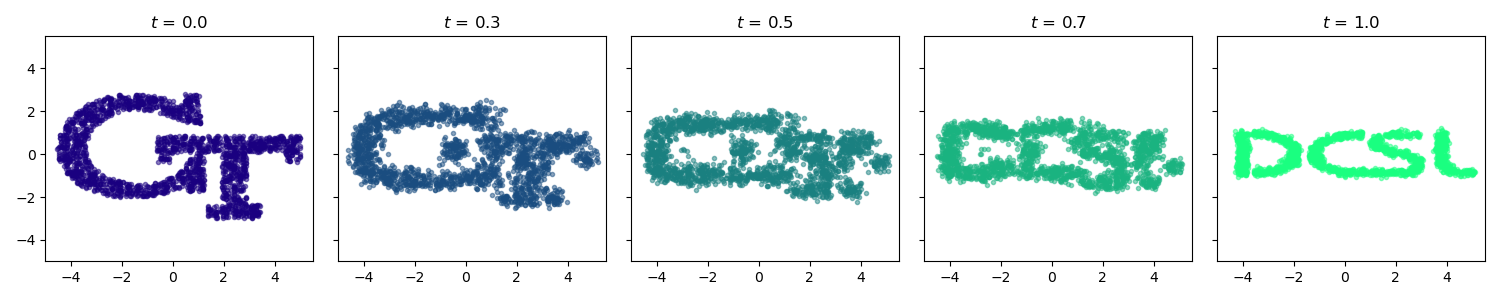
\includegraphics[ width=1. \textwidth]{figures/GT2DCSL_noisy.png}
    \caption{GT to DCSL distribution steering with zero prior dynamics and $\epsilon=0.1$.}
    \label{fig:GT2DCSL}
\end{figure*}

We first test the algorithm in 2D toy problems, starting from the case where the boundary mixture models are known explicitly.
The resulting flows are illustrated in Figure \ref{fig:GMM2D} for a Gaussian-to-Gaussian Mixture problem for various levels of noise.
To study the optimality of the proposed approach, we evaluate the resulting transport cost for policy \eqref{lambda_pol} for each noise level and compare it with the upper bound from \eqref{OTcost}.
Additionally, we benchmark our results against two state-of-the-art methods: Diffusion Schrödinger Bridge (DSB) \citep{de2021diffusion} and Diffusion Schrödinger Bridge Matching (DSBM) \citep{shi2023diffusion}. 
The exact hyper parameters for the experiments are presented in Appendix \ref{App:exp_details}.
The results are shown in Table~\ref{tab:jensen_gap}.
For the zero-noise case, DSB and DSBM are not applicable. Instead, we computed the true optimal transport cost using 10,000 samples from the boundary distributions via the POT library \citep{flamary2021pot}.

\begin{figure}[htb]
    \centering
    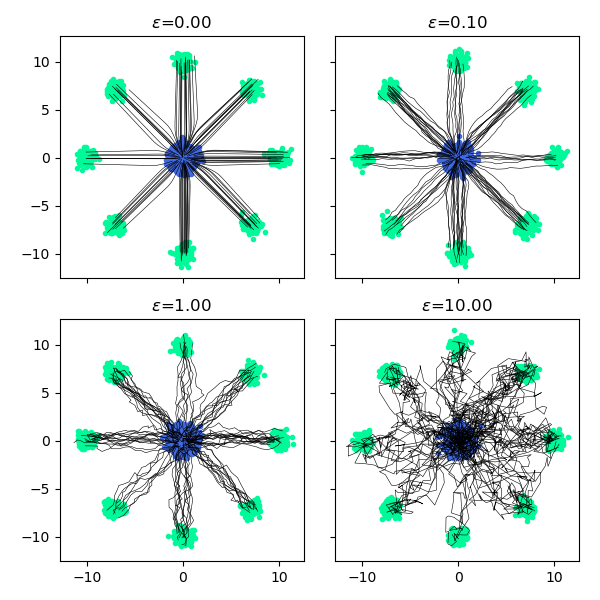
\includegraphics[width=1.\linewidth]{figures/2D_GMM.png}
    \caption{\textcolor{RoyalBlue}{Gaussian} to \textcolor{ForestGreen}{8-Gaussians} to with no prior dynamics.}
    \label{fig:GMM2D}
\end{figure}

To test the performance on problems with boundary distributions available only through samples, we test the algorithm on the distributions depicted in Figure~\ref{fig:GT2DCSL}. 
To use the proposed approach, we pre-fit GMMs with 100 components in the initial and terminal distributions using the Expectation maximization (EM) algorithm \citep{pedregosa2011scikit}. 

\begin{table} [!ht]
    \caption{Transport cost comparison.}
    \label{tab:jensen_gap}
    \setlength{\tabcolsep}{3pt}
    \centering
    \begin{tabular}{|c|c|c|c|c|c|}
    \hline
        $\epsilon$ & $J_{\mathrm{GMM}}$  \eqref{GMM_SB:cost} & $ J_{\mathrm{OT}}$  \eqref{OTcost}  & DSBM & DSB & OT\\
    \hline
        0   &   89.45   & 100.06  & -  & - & 84.87 \\
    \hline
        0.1 &   89.32   & 100.15  & 84.26 & 98.62 & -\\
    \hline
        1   &   89.28   & 102.28  &  131.50 & 100.82 & -\\
    \hline
        10   &  116.60  & 162.13  & 133.04 & 244.31 & -\\
    \hline
    \end{tabular}
\end{table}
% OT cost 84.87
% \todo{Implement one neural IPF method and a bridge matching method for solving the SB and add values in Table 1 for comparison. }
%
%
\subsection{Problems with LTI prior dynamics} \label{LTI_exps}
%
\begin{figure} 
    \centering
    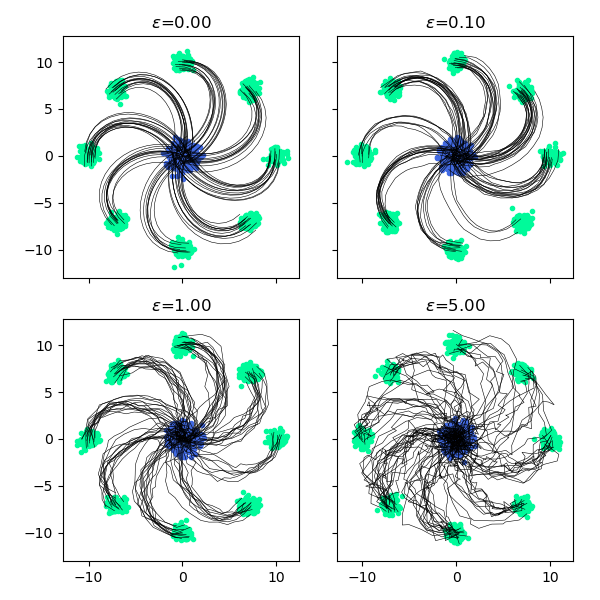
\includegraphics[width=0.9\linewidth]{figures/4D_GMM.png}
    \caption{\textcolor{RoyalBlue}{Gaussian} to \textcolor{ForestGreen}{8-Gaussians}  with LTI prior dynamics.}
    \label{fig:GMM4D}
\end{figure}
%
To test the algorithm on more complicated dynamical systems, we use the 4-dimensional Linear Time-Invariant (LTI) system 
\begin{equation} \label{LTI}
    \d x_t = A x_t \, \d t + B u_t \, \d t + D \, \d w,
\end{equation}
with
\begin{equation*}
    A = \begin{bmatrix} 2S &  I_2 \\ S & 0_2 \end{bmatrix},\, S = \begin{bmatrix} 0 &  -1 \\ 1 & 0 \end{bmatrix}, \, B = \begin{bmatrix} 0 \\ I_2  \end{bmatrix}, \,  D = \epsilon I_4 ,
\end{equation*}
and boundary distributions 
\begin{subequations}\label{ex2GMMs}
\begin{align} 
    & \rho_i = \sum_{k=0}^8 \frac{1}{8} \N( \left[ 10 \cos(k \pi/4); 10 \sin(k \pi/4); 0; 0\right], 0.4 I_4), \\
    & \rho_f = \N(0_4, 0.4 I_4).
\end{align}
\end{subequations}
%
We note that solving problem \eqref{GMM_SB} with the dynamical system \eqref{LTI} in place of \eqref{GMM_SB:dyn} is not currently solvable using any mainstream neural SB solvers because the stochastic disturbance $\d w$ in \eqref{LTI} does not enter through the same channels as the control signal $u_t$ and the state $x_t$.
The only available method to solve this problem is detailed in \citep{chen2016optimal}, which, however, assumes access to the solution of the static EOT problem \eqref{EOT} with
boundary distributions \eqref{ex2GMMs}, and a closed form of the probability density transition kernel included by the dynamical system \eqref{LTI} for $u_t \equiv 0$.
% \begin{equation}
%     \rho_i = \sum_{k=0}^8 \frac{1}{8} \N( \left[ 10 \cos(k \pi/4); 10 \sin(k \pi/4); 0; 0\right], 0.4 I_4), \quad \rho_f = \N(0_4, 0.4 I_4)
% \end{equation}
The results of our approach are illustrated in Figure~\ref{fig:GMM4D}.
%
%
\subsection{Performance on EOT benchmarks}
%
%
%
To further evaluate the optimality of the proposed approach, we tested the algorithm on the Entropic Optimal Transport benchmark detailed in \citep{gushchin2023building}.
The benchmark provides a pair of boundary test distributions $\rho_i, \rho_f$ (see Figure \ref{fig:building}), where $\rho_i$ is a scaled Normal distribution and $\rho_f$ is a mixture-like distribution whose density cannot be calculated exactly but is defined implicitly through an optimal conditional transport plan $\pi^*(x_1 \vert x_0)$, which is a Gaussian Mixture Model and is known in closed form.

\begin{figure}[htb]
    \centering
    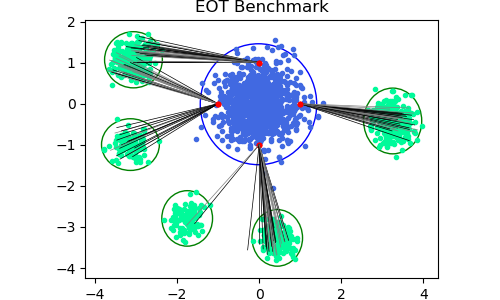
\includegraphics[width=0.9\linewidth]{figures/gwtf_benchmark.png}
    \caption{2D EOT benchmark boundary distributions, from \citep{gushchin2023building}.}
    \label{fig:building}
\end{figure}

For the pair $\rho_i, \rho_f$, the optimal policy solving \eqref{SB} can be calculated explicitly, allowing for direct comparisons with our approach.
%
The metric we use to measure the optimality of our approach is the 
Bures-Wasserstein Unexplained Variance Percentage ($\mathrm{cB}\sW\mbox{-}\mathrm{UVP}$) \citep{gushchin2023building}, defined by
\begin{subequations}
\begin{align*}
& \mathrm{cB}\sW\mbox{-}\mathrm{UVP}(\pi, \pi^*) \triangleq  \nonumber \\
& \frac{100\%}{\frac{1}{2} \mathrm{Var}(\rho_1) } \int \mathrm{B}\sW_2^2(\pi(x_1|x_0) \| \pi^*(x_1|x_0)) \rho_0(x_0) \, \d x_0,
\end{align*}
\end{subequations}
which measures the distance between conditional transport plans, evaluated using the Bures-Wasserstein metric. 

To use the method of \cite{gushchin2023building}, we first obtain samples from the two boundary test distributions and then fit mixture models on them using EM.
We then deploy policy \eqref{lambda_pol}, and report the values of the $\mathrm{cB}\sW\mbox{-}\mathrm{UVP}$ index between the known optimal conditional transport plan $\pi^*(x_1\vert x_0)$, and the conditional transport plan resulting from the integration of the policy \eqref{lambda_pol}.
The results are reported in Table \ref{tab:benchmark} for problems of various dimensions and noise levels.
We note that although the distributions described in \cite{gushchin2023building} are not, in general, mixture models, they can be closely approximated as such.
Therefore, the $\mathrm{cB}\sW\mbox{-}\mathrm{UVP}$  values reported in Table \ref{tab:benchmark} are partly due to the potential suboptimality of \eqref{lambda_pol}, and partly due to the mismatch between the true and the mixture model distributions.
%
Nonetheless, Table~\ref{tab:benchmark} places our approach among the best scoring methods for problems with boundary distributions that are mixture modes or can be closely approximated as such (see Table~5 in \citep{gushchin2023building}  for the scores of most widely used Neural Network methods for solving the SB problem)
%
% \panos{why don't we include the scores here for comparison? It is difficult to compare when the only scores in Tanble 2 are  our own}
%
while requiring virtually no training other than solving the linear program \eqref{fleet_OT} and fitting the mixture models to the data if those are not explicitly known beforehand. 

\begin{table}
    \caption{ $\mathrm{cB}\sW\mbox{-}\mathrm{UVP}$ metric for EOT benchmarks for various noise levels and problem dimensions.}
    \label{tab:benchmark}
    \centering
    \begin{tabular}{|c|c|c|c|c|}
\hline
                        & $d=2$ &$d=16$ &$d=64$ &$d=128$ \\
\hline
        $\epsilon=0.1$  &  10.35 & 14.68  & 29.20 & 11.83 \\
\hline
        $\epsilon=1.0$  &  5.78  & 7.20   & 6.93  & 6.38 \\
\hline
        $\epsilon=10$   &  0.16  & 0.28   & 1.43  & 2.77 \\
\hline
    \end{tabular}
\end{table}
%
\begin{figure*}[!ht]
    \centering
    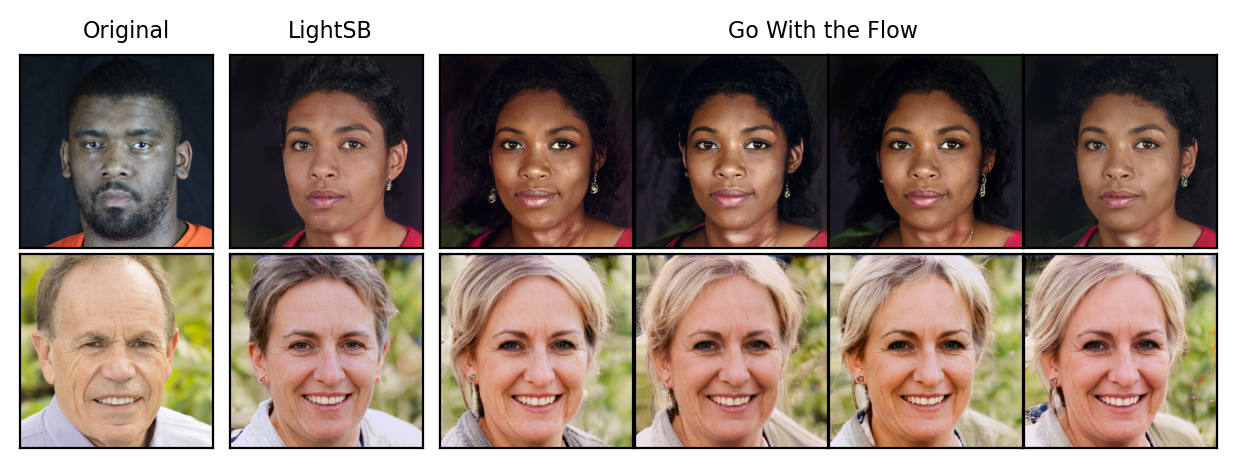
\includegraphics[width=1 \linewidth]{figures/M2F.png}
    \caption{Man to woman image translation. The first column contains the original images, the second column contains the translated image using the baseline method \cite{korotin2024light}, and the last contains 4 samples from the transformed images using the proposed approach with $\epsilon=0.1$.}
    \label{fig:M2F}
\end{figure*}
%
\begin{figure*}[!ht]
    \centering
    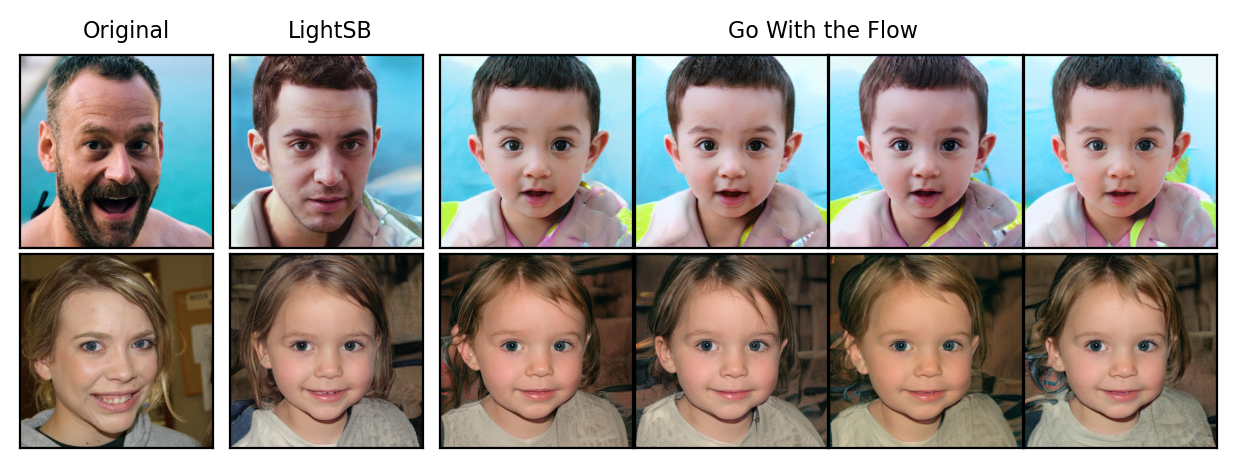
\includegraphics[width=1\linewidth]{figures/A2C.png}
    \caption{Adult to Children image translation. The first column contains the original images, the second column contains the translated image using the baseline method \cite{korotin2024light}, and the last contains 4 samples from the transformed images using the proposed approach with $\epsilon=0.1$.}
    \label{fig:A2C}
\end{figure*}
%
\subsection{Image-to-Image translation} \label{I2I_trans}
%
%
Although Mixture Models are not designed to capture high-dimensional distributions such as those of images, following \citep{korotin2024light} we use our algorithm in the latent space of an autoencoder to perform a man-to-woman and adult-to-child image translation task. 
We use the pre-trained ALAE autoencoder \citep{pidhorskyi2020adversarial} trained on the FFHQ \citep{karras2019style}.
% dataset containing 70K faces, split into a 60K training and a 10K validation set. 
The latent space of the autoencoder is 512-dimensional.
We start by fitting a 10-component mixture model to the embeddings of each image class using Scikit's \citep{pedregosa2011scikit} default EM algorithm with diagonal covariance matrices to facilitate matrix inversions in the Gaussian to Gaussian policy calculations \eqref{GSB_sol}, and then apply the mixture policy \eqref{lambda_pol}. 
The results are illustrated in Figures \ref{fig:M2F} and \ref{fig:A2C}.
% Compared with the LightSB solver, our approach performs more aggressive changes in the image features, which we believe is due to the use of the Expectation Maximization algorithm for the GMM pre-fitting, which is known to be less prone to converge to locally optimal values, compared to LightSB's Maximum likelihood objective.
To test how well the generated images match the features of the given target distribution, we calculate the Fréchet inception distance (FID) scores \cite{heusel2017gans} between the actual and the generated images of a given class, using 10000 samples from each distribution.
The FID scores correspond to the empirical Bure-Wasserstein distance between the images of the two classes, evaluated in the latent space of the Inception network. 
To further test how close the transformed images are to the target class, we also calculate the empirical Bure-Wasserstein distance between the transformed images and the real images of the target class, directly in the latent space of the ALAE autoencoder, since this is the space our algorithm is trained in.
We compare against two state-of-the-art lightweight SB solvers, LSB \cite{korotin2024light} and LSBM \cite{gushchin24light}, and present the results in Tables \ref{FID:M2W}, \ref{FID:A2C}.
\begin{table}[!ht]
    \centering
    \begin{tabular}{l|cc}
        M$\rightarrow$W &  FID  &   ALAE-B$\mathcal{W}_2$  \\
        \hline
        LSB             &  4.94     & 28.9  \\
        LSBM            &  4.98     & 28.3  \\
        GMMflow (ours)  &  3.04     & 9.3   \\
    \end{tabular}
    \caption{Man to Woman FID comparison}
    \label{FID:M2W}
\end{table}

\begin{table} [!ht]
    \centering
    \begin{tabular}{l|cc}
          A$\rightarrow$C   & FID &  ALAE-B$\mathcal{W}_2$  \\
        \hline
        LSB                 &  6.62   &  31.00  \\
        LSBM                &  6.61   &  30.99  \\
        GMMflow (ours)      &  3.50   &  8.54   \\
    \end{tabular}
    \caption{Adult to Child FID comparison}
    \label{FID:A2C}
\end{table}

Qualitatively, our algorithm performs more aggressive feature changes compared to the baseline method, as illustrated in Figures \ref{fig:M2F}, \ref{fig:A2C}. 
On a quantitative level, the features of the transformed images better capture the true distribution of the features of a given target class, given the almost 40\% better FID scores and 65\% better ALAE-B$\mathcal{W}_2$ scores provided in tables \ref{FID:M2W}, \ref{FID:A2C}.
We believe that this significant performance increase is due to the fact that our algorithm leverages the Expectation Maximization algorithm for the GMM pre-fitting, which is less prone to converge to locally optimal values, compared to LightSB's Maximum likelihood objective, or the LSBM's bridge matching objective.
We further remark that our approach takes 63\% less time to train, as noted in Table \ref{tab:speed}, Appendix \ref{expDetails_Im}.

%
\section{Conclusion}
This paper introduces a novel, efficient method for solving the Schrödinger Bridge problem with Gaussian Mixture Model boundary distributions by utilizing a mixture of conditional policies, each solving a Gaussian bridge subproblem. 
Unlike traditional methods that rely on computationally expensive training of neural networks, which approximately solve high-dimensional non-convex optimization problems, our approach approximates the optimal policy by solving a low-dimensional linear program exactly.
Furthermore, the method extends naturally to more general classes of dynamical systems, such as controllable Linear Time-Varying (LTV) systems. 
Through various experiments, including image-to-image translation tasks, we demonstrate that our outperforms state-of-the-art methods for solving the same task, while requiring minimal computational effort (i.e., no training), highlighting its potential for practical applications in diverse fields, from generative modeling to control theory.
% Unlike conventional approaches that often require computationally expensive training or simulations, 

\subsection*{Acknowledgements}
% 
Support for this work has been provided by 
ONR award N00014-18-1-2828 and NASA ULI award \#80NSSC20M0163.
This article solely reflects the opinions and conclusions of its authors and not of any NASA entity. 
George Rapakoulias acknowledges financial support from the A. Onassis Foundation Scholarship.
% \clearpage
\bibliographystyle{iclr2025_conference}
\bibliography{refs}

% \clearpage
% \onecolumn
% \begin{enumerate}

% \clearpage
%  \item For all models and algorithms presented, check if you include:
%  \begin{enumerate}
%    \item A clear description of the mathematical setting, assumptions, algorithm, and/or model. \textcolor{blue}{Yes}
%    \item An analysis of the properties and complexity (time, space, sample size) of any algorithm. \textcolor{blue}{No}
%    \item (Optional) Anonymized source code, with specification of all dependencies, including external libraries. \textcolor{blue}{Yes}
%  \end{enumerate}


%  \item For any theoretical claim, check if you include:
%  \begin{enumerate}
%    \item Statements of the full set of assumptions of all theoretical results. \textcolor{blue}{Yes}
%    \item Complete proofs of all theoretical results. \textcolor{blue}{Yes}
%    \item Clear explanations of any assumptions. \textcolor{blue}{Yes}
%  \end{enumerate}


%  \item For all figures and tables that present empirical results, check if you include:
%  \begin{enumerate}
%    \item The code, data, and instructions needed to reproduce the main experimental results (either in the supplemental material or as a URL). \textcolor{blue}{Yes}
%    \item All the training details (e.g., data splits, hyperparameters, how they were chosen). \textcolor{blue}{Yes}
%          \item A clear definition of the specific measure or statistics and error bars (e.g., with respect to the random seed after running experiments multiple times). \textcolor{blue}{Yes}
%          \item A description of the computing infrastructure used. (e.g., type of GPUs, internal cluster, or cloud provider). \textcolor{blue}{Yes}
%  \end{enumerate}

%  \item If you are using existing assets (e.g., code, data, models) or curating/releasing new assets, check if you include:
%  \begin{enumerate}
%    \item Citations of the creator If your work uses existing assets. \textcolor{blue}{Yes}
%    \item The license information of the assets, if applicable. \textcolor{blue}{Yes}
%    \item New assets either in the supplemental material or as a URL, if applicable. \textcolor{blue}{Yes}
%    \item Information about consent from data providers/curators.\textcolor{blue}{Not Applicable}
%    \item Discussion of sensible content if applicable, e.g., personally identifiable information or offensive content. \textcolor{blue}{Not Applicable}
%  \end{enumerate}

%  \item If you used crowdsourcing or conducted research with human subjects, check if you include:
%  \begin{enumerate}
%    \item The full text of instructions given to participants and screenshots. \textcolor{blue}{Not Applicable}
%    \item Descriptions of potential participant risks, with links to Institutional Review Board (IRB) approvals if applicable. \textcolor{blue}{Not Applicable}
%    \item The estimated hourly wage paid to participants and the total amount spent on participant compensation. \textcolor{blue}{Not Applicable}
%  \end{enumerate}

%  \end{enumerate}


\onecolumn
\appendix

\setcounter{equation}{0}
\renewcommand{\theequation}{A.\arabic{equation}}

% \panos{should we re-start the equation numbering in the Appendix, i.e., (A.1), (A.2), etc?}

\section{Proofs} \label{App_proofs}

All proofs are carried out for a general Linear Time-Varying (LTV)
\begin{equation} \label{LTV}
    \d x_t = A_t x_t \, \d t + B_t u(x_t) \, \d t + D_t \, \d w,
\end{equation}
where $x_t \in \sR^d, \, A_t \in \sR^{d \times d}, \, u_t \in \sR^{m}, \, B_t \in \sR^{d \times m}, \, D_t \in \sR^{d \times q}$ and $\d w$ is the $q$-dimensional Brownian increment having the properties
$\E[\d w] = \E[\dw \, \d t ] = 0 $ and $\E [\dw\t\, \dw] = \d t $.
%
The dynamical system \eqref{GMM_SB:dyn} is just a special case of \eqref{LTV}
with $A_t = 0, B_t = I, D_t = \sqrt{\epsilon} \, I$.

\subsection{The Fokker-Plank-Kolmogorov equation}

The equation describing the propagation of the distribution of the state of the dynamical system \eqref{LTV}, known as the Fokker-Plank-Kolmogorov (FPK) equation \citep{sarkka2019applied} is:
%
\begin{equation} \label{FPK}
    \frac{\partial \rho_t}{\partial t}  +  \sum_i \frac{\partial}{\partial x_i} 
    \big(  \rho_t (A_t x_t + B_t u_t(x_t)) \big) 
    - \frac{1}{2} \sum_{i,j} \frac{\partial^2}{\partial x_i \partial x_j} \big( [D_t D_t\t]_{ij} \rho_t(x_t)\big) = 0.
\end{equation}
%
This equation can be written more compactly using standard vector notation as follows
\begin{equation} \label{FPK_comp}
    \frac{\partial \rho_t}{\partial t}  +  \nabla \cdot \left( \rho_t (A_t x_t + B_t u_t(x_t)) \right) - \frac{1}{2} \tr \left( D_t D_t\t \hess(\rho_t) \right) = 0, 
\end{equation}
% \todo{change $\su$ to $\tr$...}
where $\hess(\rho_t)$ denotes the Hessian of the density with respect to the state $x_t$ at time t.
% , $\odot$ denotes the element-wise product between two matrices of the same dimensions and $\su(\cdot)$ denotes the sum of all the elements of a matrix.
In the specific case where $D_t = \sqrt{\epsilon} \, I$, equation~\eqref{FPK_comp} reduces to the well-known equation
\begin{equation}
        \frac{\partial \rho_t}{\partial t}  + \nabla \cdot \left( \rho_t (A_t + B_t u_t) \right) - \frac{\epsilon}{2} \Delta \rho_t(x) = 0,
\end{equation}
where $\Delta$ denotes the Laplacian operator.

% 
\subsection{Proof of Theorem \ref{feasibility_thm}} 

First, notice that the probability flow \eqref{rho_lambda} respects the constraint \eqref{GMM_SB:BC0}, \eqref{GMM_SB:BC1} for all feasible values of $\lambda_{ij}$, since 
\begin{subequations}
\begin{align}
    \rho_0 &= \sum_{i,j} \rho_{0|ij} \lambda_{ij} = \sum_{i,j} \N(\mu^i_0, \Sigma_0^i) \lambda_{ij} = \sum_{i} \N(\mu^i_0, \Sigma_0^i) w_i,\\
    \rho_1 &= \sum_{i,j} \rho_{1|ij} \lambda_{ij} = \sum_{i,j} \N(\mu^j_1, \Sigma_1^i) \lambda_{ij} = \sum_{j} \N(\mu^j_1, \Sigma_1^i) w_j.
\end{align}
\end{subequations}
%
Therefore, it suffices to show that the policy \eqref{lambda_pol} produces the probability flow \eqref{rho_lambda}.
Following the approach of~\cite{lipman2022flow} and \cite{liu2024generalized}, we show that the pair \eqref{lambda_pol}, \eqref{rho_lambda} satisfies the FPK equation.
% Consider the system \eqref{LTI:dyn} and its state density at time $t$ given by $\rho_t$. 
% The evolution of $\rho_t$ is given by the Fokker Plank Equation (FPK) equation \citep{sarkka2019applied}.
% Therefore, to prove Lemma \ref{lemma1}, it suffices to show that the pair $\rho_t$ in \eqref{mixture_flow} and $u_t$ in \eqref{unc_pol} satisfy the FPK. 
We start from the FPK equation describing a conditional flow and sum over all conditional variables to retrieve the unconditional flow. 
%
Specifically, given that the individual policies $u_{t|ij}$ solve the Gaussian Bridge subproblems \eqref{GSB}, the pair $\rho_{t|ij}, \, u_{t|ij}$ satisfies the FPK equation for the dynamical system~\eqref{LTV}, that is,
%
\begin{subequations}
    \begin{align}
         & \frac{\partial \rho_{t|ij}}{\partial t} + \nabla \cdot \left( \rho_{t|ij}(A_t x_t + B_t u_{t|ij}) \right) - \frac{1}{2} \tr \left( D_t D_t\t \hess(\rho_{t|ij}) \right) = 0, \\
         % 
         & \nonumber \\
         & \textrm{\! Multiplying with $\lambda_{ij}$ and summing, we obtain} \nonumber \\
         & \nonumber \\
         %
         &  \sum_{i,j} \lambda_{ij} \left[ \frac{\partial \rho_{t|ij}}{\partial t} + \nabla \cdot \left( \rho_{t|ij}(A_t x_t + B_t u_{t|ij} ) \right) - \frac{1}{2} \tr \left( D_t D_t\t \hess(\rho_{t|ij}) \right) \right] = 0,  \\
         % 
         & \frac{\partial}{\partial t} \left( \sum_{i,j} \rho_{t|ij} \lambda_{ij} \right) + \nabla \cdot \left(  A_t x_t \sum_{i,j} \rho_{t|ij} \lambda_{ij} + B_t \sum_{i,j} u_{t|ij} \rho_{t|ij} \lambda_{ij}  \right) - \frac{1}{2} \tr \left( D_t D_t\t \hess \left( \sum_{i,j} \rho_{t|ij} \lambda_{ij} \right) \right) = 0.  \label{feas:step3} \\
          % 
         & \frac{\partial \rho_t}{\partial t} + \nabla \cdot \left( \rho_t \left( A_t x_t + B_t \sum_{ij} u_{t|ij}\frac{\rho_{t|ij} \lambda_{ij} }{\sum_{i,j} \rho_{t|ij} \lambda_{ij}} \right) \right) - \frac{1}{2} \tr \left( D_t D_t\t \hess(\rho_{t}) \right) = 0, \\
         %
         & \nonumber \\
         & \textrm{\! and finally,} \nonumber \\
         & \nonumber \\
         %
         & \frac{\partial \rho_t}{\partial t} + \nabla \cdot \left( \rho_t (A_t x_t + B_t u_t) \right) - \frac{1}{2} \tr \left( D_t D_t\t \hess(\rho_{t}) \right) = 0.
    \end{align}
\end{subequations}
 
%
\subsection{Proof of Theorem \ref{OT_thm}}

It suffices to show that the cost \eqref{GMM_SB:cost} is upper bounded by the cost of 
\eqref{OTcost}.
Substituting policy \eqref{lambda_pol} to the cost \eqref{GMM_SB:cost} we obtain
\begin{subequations}
\begin{align}
     J_{\mathrm{GMM}} =  & \E_{x_t \sim \rho_t} \left[ \int_{0}^{1}{ \left\| \sum_{i,j} {u_{t|ij}(x) \frac{ \rho_{t|ij}(x)\lambda_{ij}}{\sum_{i,j} \rho_{t|ij}(x) \lambda_{ij}}} \right\|^2 \d t} \right] \\
    %
    = & \int_{0}^{1} \int { \rho_t \left\| \sum_{i,j} {u_{t|ij}(x) \frac{ \rho_{t|ij}(x)\lambda_{ij}}{\sum_{i,j} \rho_{t|ij}(x) \lambda_{ij}}} \right\|^2 \, \d x \, \d t} \label{step2} \\
    % 
    \leq & \int_{0}^{1} \int { \rho_t \frac{ \sum_{i,j} \left\|u_{t|ij}(x)\right\|^2 \rho_{t|ij}(x)\lambda_{ij}}{\sum_{i,j} \rho_{t|ij}(x) \lambda_{ij}}  x \, \d t}  \label{jensen} \\
    %
    = & \int_{0}^{1}  \int { \sum_{i,j} \left\|u_{t|ij}(x)\right\|^2 \rho_{t|ij}(x) \lambda_{ij}}  \, \d x \, \d t \\
    %
    = & \sum_{i,j} \lambda_{ij} \E_{x \sim \rho_{t|ij}} \left[
 \int_{0}^{1} { \left\|u_{t|ij}(x)\right\|^2}  \, \d t \right] \\
    %
    = & \sum_{i,j} \lambda_{ij} J_{ij} = J_{\mathrm{OT}}
\end{align}
\end{subequations}
where \eqref{step2} is due to Fubini's theorem 
\cite[Theorem~6.1]{wheeden1977measure} and \eqref{jensen} makes use of the discrete version of Jensen's inequality \cite[Theorem~7.35]{wheeden1977measure}.

% \section{The limit of small Covariances} \label{AppB}
% \george{this needs some refinement. I will finish it in the next couple of days.}

% Theorem \ref{OT_thm} provides an upper bound for Problem \eqref{GMM_SB}, but does not quantify the gap between the optimal solutions of the two problems. 
% To this end, an alternative approach is considered, based on properties of the Schr\"{o}dinger bridge problem. 
% For the case of trivial dynamics (i.e. $A = 0, B = D = I$) minimizing the cost function \eqref{GMM_SB:cost} is equivalent to the KL-divergence of the path measures between the controlled and uncontrolled process, i.e.
% \begin{equation} \label{pathKL}
%     \min_{\mathcal{P} \in \mathbb{D}} \mathrm{D}_{\mathrm{KL}}( \mathcal{P} \| \mathcal{Q})
% \end{equation}
% where $\mathcal{P}, \mathcal{Q}$ are the path measures of the controlled and uncontrolled processes respectively, and $\mathbb{D}$ is the set of path measures with boundary marginals $\rho_i, \rho_f$ at times $t = 0, t =1$ \citep{chen2021stochastic, leonard2014survey}. 
% Using the disintegration property of path measures, one can show that minimizing \eqref{pathKL} is equivalent to minimizing the KL divergence between the joint initial-final distributions of the controlled and uncontrolled processes.
% Specifically, when $\mathcal{Q}$ is a Wiener process, cost function \eqref{pathKL} is equivalent to 
% \begin{equation} \label{transp_opt}
%     \min_{\rho_{01} \in \Pi(\rho_i, \rho_f)} \int \frac{\| x_0 - x_1 \|^2}{2} \rho_{01}(x_0, x_1) d x_0 d x_1 + \epsilon \int \rho_{01} \log \rho_{01} \d x_0 \d x_1
% \end{equation}
% where $\Pi(\rho_i, \rho_f)$ is the set of all joint distributions with marginals $\rho_i, \rho_f$ \citep{chen2021stochastic}.
% When $\rho_i, \rho_f$ are empirical distributions, i.e. a weighted sum of Dirac delta functions, the transport plan takes the form 
% %
% \begin{equation} \label{delta_transp}
%     \rho_{01}(x_0, x_1) = \sum_{i,j} \lambda_{ij} \delta_{i}(x_0) \delta_{j}(x_1)
% \end{equation}
% %
% where $\lambda_{ij} \geq 0$ and $\delta_i(x_0), \delta_j(x_1)$ are Dirac delta functions centered at $x_0^i, x_1^j$ respectively.
% Substituting \eqref{delta_transp} in \eqref{transp_opt} and using the sifting property of the delta function, one can show that the problem of finding the optimal transport plan amounts to the calculation of $\lambda_{ij}$ through the discrete EOT problem
% \begin{equation} \label{EOT_plan}
%     \min_{\lambda_{ij}} \sum_{i,j} \frac{\| x^i_0 - x^j_1 \|}{2} \lambda_{ij} + \epsilon \sum_{i,j} \lambda_{ij} \log \lambda_{ij}  + c = \min_{\Lambda} \tr (C\t \Lambda) + \epsilon H(\Lambda) + c.
% \end{equation}
% where $C_{ij}=\|x_0^i - x_1^j\|^2$ and $\Lambda_{ij} = \lambda_{ij}$, $c$ is independent of $\Lambda$, and $H(\cdot)$ is the discrete entropy of the transport plan \citep{peyre2017computational}.

% In the case where the boundary distributions are mixture models, the calculations carries through with two assumptions:
% \begin{enumerate}
%     \item The transport plan between the initial and final distribution can be expressed as  
% \begin{equation}
%     \rho_{01}(x_0, x_1) = \sum_{i,j} \lambda_{ij} \rho^{i}_0(x_0) \rho^{j}_1(x_1)
% \end{equation}
% which holds if the Gaussians components in each mixture have small enough covariances. 
% %
% \item The components in each mixture are approximately disjoint, meaning that $\rho_i^0(x) \rho_j^0(x)  \approx 0 \; \forall \; i \neq j, \; x \in \sR^n$.
% \end{enumerate}

% Then, expression \eqref{transp_opt} reduces to 

% \begin{subequations}
% \begin{align}
%     & \int \sum_{i,j}  \frac{\| x_0 - x_1 \|^2}{2} \lambda_{ij} \rho_i(x_0) \rho_j(x_1) \d x_0 \d x_1 \nonumber \\
%     & + \epsilon \int \sum_{i,j} \lambda_{ij} \rho_i(x_0) \rho_j(x_1) \log \left( \sum_{i,j} \lambda_{ij} \rho_i(x_0) \rho_j(x_1) \right) \d x_0 \d x_1 \\
%     & = \sum_{i,j}  \frac{\| \mu^i_0 - \mu^j_1 \|^2}{2} \lambda_{ij} +  \epsilon \int \sum_{i,j} \lambda_{ij} \rho_i(x_0) \rho_j(x_1) \log \left( \lambda_{ij} \rho_i(x_0) \rho_j(x_1) \right) \d x_0 \d x_1 \\
%     & = \sum_{i,j}  \frac{\| \mu^i_0 - \mu^j_1 \|^2}{2} \lambda_{ij} +  \epsilon \sum_{i,j} \lambda_{ij}  \log (\lambda_{ij}) +  \int \sum_i w_0^i \rho_0^i(x_0) \log \left( \rho_0^i(x_0) \right) \d x_0 \nonumber \\
%     & + \int \sum_j \rho_1^j(x_1) \log \left( \rho_1^j(x_1) \right) \d x_1 \\
%     & = \tr (C\t \Lambda) + \epsilon H(\Lambda) + \epsilon(H(\rho_0) + H(\rho_1)).
% \end{align}
% \end{subequations}
% This shows that under these assumptions, the optimal transport plan $\lambda_{ij}$ between components of the mixture can be calculated exactly by solving a discrete entropic optimal transport problem, as in the case of an empirical distribution. 

\section{Experiment Details} \label{App:exp_details}

\subsection{2D Problems}

To compare our approach with state-of-the-art Neural SB Solvers we used the original implementations of the DSB\footnote{\url{https://github.com/JTT94/diffusion_schrodinger_bridge}} \citep{de2021diffusion} and DSBM\footnote{\url{https://github.com/yuyang-shi/dsbm-pytorch}} \citep{shi2023diffusion} algorithms and report the results in 
Table~\eqref{tab:benchmark}. 
%
The network architecture used for both algorithms is the fully connected DNN 
of~\cite{de2021diffusion} with $128$-dimensional sinusoidal temporal encodings, 256 neurons in the encoder layer, $\{256, 256\}$ neurons in the decoder layers and SiLU activation functions \citep{hendrycks2016gaussian}.
%
\begin{figure}[htb]
    \centering
    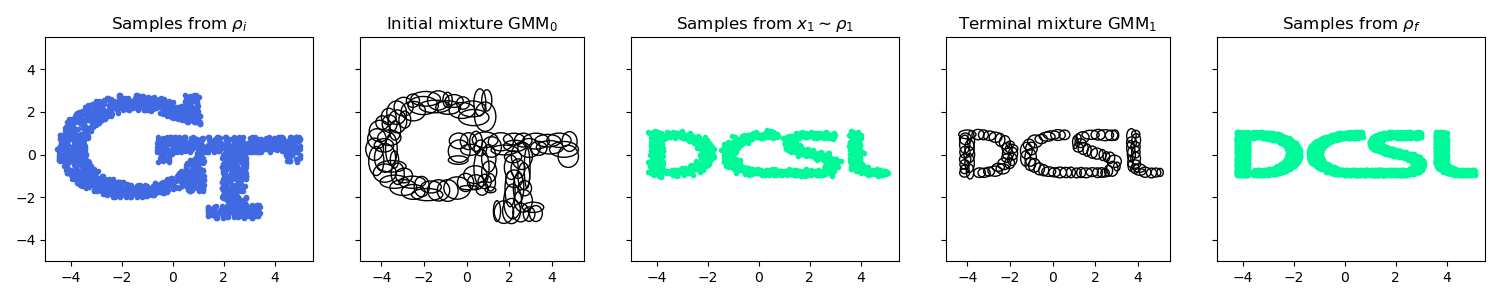
\includegraphics[width=1.\linewidth]{figures/GT2DCSL_noisy_comparison.png}
    \caption{\textcolor{RoyalBlue}{GT} to \textcolor{ForestGreen}{DCSL} distribution steering details.}
    \label{fig:AI2STAT_details}
\end{figure}
%

\subsection{Problems with LTI prior dynamics}

To solve the Gaussian Bridge sub-problems with a dynamical system of the form \eqref{LTI} we use the discrete-time convex formulation 
of~\cite{rapakoulias2023discrete}. 
We also include a brief overview of the method in Appendix~\ref{App:OCS}. 
Each continuous-time Gaussian Bridge is discretized (in the temporal dimension) into 101 steps over uniform intervals of size $\Delta t = 0.01$. 
We used MOSEK \citep{aps2020mosek} to solve the resulting semidefinite programs. 

% \subsection{Performance on EOT Benchmarks}

\subsection{Image-to-Image translation} \label{expDetails_Im}
%
To better evaluate the performance of the proposed approach in the task of Image-to-Image translation, we provide further examples in Figures \ref{fig:m2f_extended}, \ref{fig:a2c_extended}. 
We also provide approximate training and inference times for our approach for the two examples in subsection \ref{I2I_trans} and compare them with the training and inference times of LightSB in Table \ref{tab:speed}.
For our approach, training time consists of the the time required to fit the GMMs in the encodings of the FFHQ dataset for the two boundary distributions, and the solution of the linear program \eqref{fleet_OT}. 
As inference time, we consider the time taken for the integration of the SDE (or ODE for $\epsilon=0$) \eqref{GMM_SB:dyn} with the mixture policy \eqref{lambda_pol}.
We observe that while inference time is small for solving the deterministic (optimal transport) problem, i.e. for $\epsilon=0$, integrating the stochastic dynamical system for positive values of $\epsilon$ requires more time due the small time step required for SDE integration.
%
The quality of the produced images was not found to be affected by this parameter, implying that $\epsilon=0$ could be used for fast, deterministic inference, while a positive value of $\epsilon$ will allow for some randomness in the generated images.  
We also note that the faster training time for our approach is mainly due to the very fast convergence of the EM algorithm, which is also less likely to converge to local minima, compared to the standard maximum likelihood method for fitting distribution to data. 
All tests were conducted on a desktop computer with RTX 3070 GPU. 
\begin{table} [!ht]
    \centering
    \begin{tabular}{|c|c|c|c|}
    \hline
                 & Training [s]  &  Inference ($\epsilon=0$) [s], & Inference ($\epsilon=0.1$) [s]\\
    \hline
         LightSB\tablefootnote{\cite{korotin2024light}} & 57 &  -  & 0.02\\
    \hline
         Ours    & 21 & 0.7 & 6.5\\
    \hline
    \end{tabular}
    \caption{Training and inference time comparison with state of the art. Inference time is measured for a batch of 10 images.}
    \label{tab:speed}
\end{table}
%
\section{Gaussian Bridge for Linear Time-Varying systems} \label{App:OCS}
%
\setcounter{equation}{0}
\renewcommand{\theequation}{C.\arabic{equation}}
%
In this section, we briefly review the methods available in the literature to solve the Gaussian Bridge problem with general LTV dynamics of the form \eqref{LTV}.
That is, we consider the problem 
\begin{subequations} \label{OCS}
\begin{align}
& \min_{u \in \mathcal{U}} \; \E \left[ \int_{0}^{1}{ \| u_t(x) \|^2 \d t} \right], \label{OCS:cost} \\
&     \d x_t = A_t x_t \, \d t + B_t u(x_t) \, \d t + D_t \, \d w, \label{OCS:dyn} \\
& x_0 \sim \N(\mu_i, \Sigma_i), \quad x_1 \sim \N(\mu_f, \Sigma_f). \label{OCS:BC}
\end{align}
\end{subequations}
The solution of problem \eqref{OCS} is used to solve the Gaussian Bridge problem for the example in Section~\ref{LTI_exps} and is relevant to applications with prior dynamics of more general structure such as mean field games \citep{bensoussan2016linear} and large multi-agent control applications~\citep{saravanos2023distributed}.
%
The existence and uniqueness of solutions for problem \eqref{OCS} are studied in \citep{chen2015optimal, liu2022optimal, liu2024reachability}.
Since the state of \eqref{OCS:dyn} remains Gaussian throughout the steering horizon, i.e., $x_t \sim \N(\mu_t, \Sigma_t)$, the problem simplifies to that of the control of the first two statistical moments of the state, namely the mean $\mu_t$ and the covariance $\Sigma_t$. 
Using a control policy parametrization of the form 
\begin{equation} \label{feedback_LTI}
    u_t(x) = K_t(x-\mu_t) + v_t,
\end{equation}
allows for the decoupling of the propagation equations for the mean and covariance of the state. 
More specifically, applying \eqref{feedback_LTI} to \eqref{OCS:dyn}, the equations describing the propagation of $\mu_t$ and $\Sigma_t$ yield
\begin{subequations}
\begin{align}
& \dot{\Sigma}_t = (A_t + B_t K_t) \Sigma_t+ \Sigma_t (A_t + B_t K_t) \t + D_t D_t\t, \label{Cov_prop}\\
& \dot{\mu}_t = A_t \mu_t + B_t v_t. \label{mean_prop}
\end{align}
\end{subequations}
%
%
Expanding the expression \eqref{Cov_prop} and performing the change of variables $U_t = \Sigma_t K_t$, we obtain 
\begin{equation} \label{S_d_trans}
    \dot{\Sigma}_t = A_t \Sigma_t A_t\t + B_t U_t + U_t\t B_t\t + D_t D_t\t,
\end{equation}
which is linear in $U_t, \Sigma_t$.
Furthermore, substituting \eqref{feedback_LTI} to the cost function \eqref{OCS:cost}, it simplifies to  
\begin{equation} \label{cost_reform}
    \E \left[ \int_{0}^{1}{ \| u_t(x) \|^2 \, \d t} \right] = \int_0^1 v_t\t v_t + \tr (K_t \Sigma_t K_t \t) \, \d t = \int_0^1 v_t\t v_t + \tr (U_t \Sigma_t^{-1} U_t \t) \, \d t.
\end{equation}
Equations \eqref{mean_prop}, \eqref{S_d_trans}, \eqref{cost_reform} can be used to reformulate problem \eqref{OCS} to a simpler optimization problem in the space of affine feedback policies, parameterized by $U_t, v_t$.
To be more precise, problem \eqref{OCS} reduces to 
\begin{subequations} \label{OCS_reform}
\begin{align}
& \min_{\mu_t, v_t, \Sigma_t, U_t} \; \int_0^1 v_t\t v_t + \tr (U_t \Sigma_t^{-1} U_t \t) \, \d t, \label{OCS_reform:cost} \\
& \dot{\Sigma}_t = A_t \Sigma_t A_t\t + B_t U_t + U_t\t B_t\t + D_t D_t\t,\label{OCS_reform:Cov} \\
& \dot{\mu}_t = A_t \mu_t + B_t v_t, \\
& \mu_0 = \mu_i, \, \Sigma_0 = \Sigma_i, \, \mu_1 = \mu_f, \, \Sigma_1 = \Sigma_f.
\label{OCS_reform:mean}
\end{align}
\end{subequations}
which can be further relaxed to a convex semi-definite program using the lossless convex relaxation~\cite{chen2015optimal2}
\begin{subequations} \label{cvx}
\begin{align}
& \min_{\mu_t, v_t, \Sigma_t, U_t} \; \int_0^1 v_t\t v_t + \tr (Y_t \t) \, \d t, \label{cvx:cost} \\
& U_t \Sigma_t^{-1} U_t \preceq  Y_t, \label{cvx:lmi} \\
& \dot{\Sigma}_t = A_t \Sigma_t A_t\t + B_t U_t + U_t\t B_t\t + D_t D_t\t,\label{cvx:cov} \\
& \dot{\mu}_t = A_t \mu_t + B_t v_t. \label{cvx:mean} \\
& \mu_0 = \mu_i, \, \Sigma_0 = \Sigma_i, \, \mu_1 = \mu_f, \, \Sigma_1 = \Sigma_f,
\end{align}
\end{subequations}
after noting that the constraint \eqref{cvx:lmi} can be cast as a Linear Matrix Inequality (LMI) using Schur's complement as 
\begin{equation*}
\begin{bmatrix} 
\Sigma_t & U_t\t \\
U_t & Y_t
\end{bmatrix} \succeq 0.
\end{equation*} 
Problem \eqref{cvx} is still infinite dimensional since the decision variables are functions of time $t \in [0, 1]$, however, it can be discretized, approximately using a first-order approximation of the derivatives in \eqref{cvx:cov}, \eqref{cvx:mean} \citep{chen2015optimal2} or exactly using a zero-order hold \citep{liu2022optimal, rapakoulias2023discrete}, and solved to global optimality using a semidefinite programming solver such as MOSEK \citep{aps2020mosek}.

\begin{figure}[!ht]
    \centering
    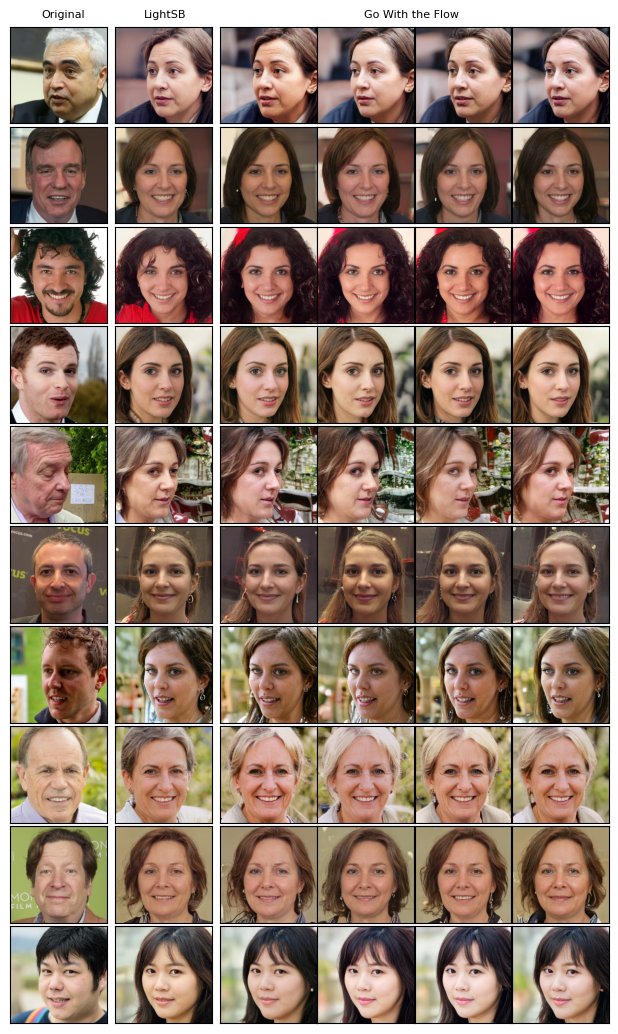
\includegraphics[width=0.7 \linewidth]{figures/M2F_extended.png}
    \caption{Further examples for the man-to-woman Image-to-Image translation task.}
    \label{fig:m2f_extended}
\end{figure}
%
\begin{figure}
    \centering
    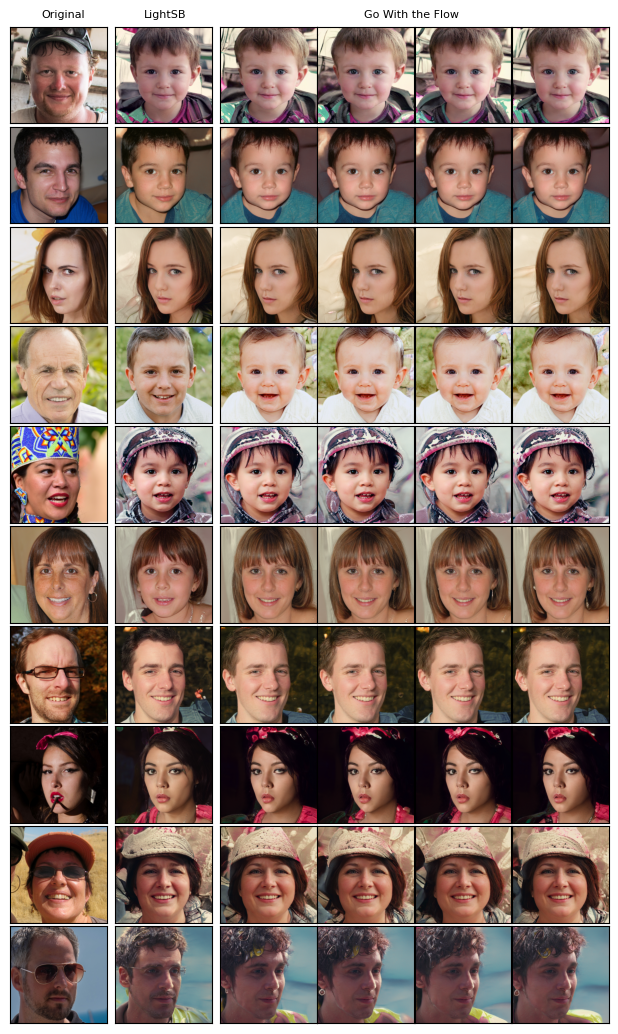
\includegraphics[width=0.7 \linewidth]{figures/A2C_extended.png}
    \caption{Further examples for the adult-to-child Image-to-Image translation task.}
    \label{fig:a2c_extended}
\end{figure}
%
% 
% \subsection{Constrained Flows}
% An important property of policy \eqref{lambda_pol} is that if the conditional policies and flows are designed to respect probabilistic constraints, these constraints will be inherited in the mixture flow. 
% This is formalized in the following statement:
% \begin{corollary}
%     Let the conditional polices $u_{t|ij}$ correspond to conditional flows $\rho_{t|ij}$ that are safe with probability $1-\delta$, i.e. $\P(x_t \in \X) > 1 - \delta$ for $x_t \sim \rho_{t|ij}$. Then, the unconditional policy \eqref{lambda_pol} is also safe. 
% \end{corollary}
% \begin{proof}
%     This is an immediate consequence of the fact that the unconditional policy \eqref{rho_lambda} generates the flow \eqref{rho_lambda}. 
%     Since the conditional flows are safe, we have: 
%     \begin{subequations}
%         \begin{align*}
%            & \P(x_t \in \X) > 1 - \delta_t \textrm{, for } x_t \sim \rho_t(x|z_i)\\
%            & \int_{x \in \X} \rho_t(x|z_i) d x > 1 - \delta_t  \\
%            & \frac{1}{N} \sum_i \int_{x \in \X} \rho_t(x|z_i) d x > \frac{1}{N} \sum_i (1 - \delta_t) \\
%            & \int_{x \in \X}  \sum_i \frac{1}{N} \rho_t(x|z_i) d x > 1 - \delta_t \\
%             & \P(x_t \in \X) > 1 - \delta_t \textrm{, for } x_t \sim \rho_t(x)
%         \end{align*}
%     \end{subequations}
% \end{proof}

% \section{Code}
% We commit to making our code publicly available by the camera-ready deadline, provided our work is accepted for publication. 

% \bibliographystyle{iclr2025_conference}
% \bibliography{refs}

\end{document}
